\documentclass{article}
\usepackage[utf8]{inputenc}
\usepackage{comment, graphicx}
\usepackage[paper=a4paper,left=2cm, right=2cm, top=2cm]{geometry}
\usepackage{amsmath}

\usepackage{comment}

\usepackage{float}
\usepackage{graphicx}
\usepackage{subfig}
\usepackage{threeparttable}
\usepackage{booktabs}
\usepackage[hang,flushmargin,bottom]{footmisc}
\usepackage{dblfloatfix}
\usepackage{array}
\usepackage{amsfonts}

\usepackage{setspace}
\setstretch{1.5}

% no indent in paragraphs
\setlength\parindent{0pt}

% no indent in enumerate
\usepackage{enumitem}

% symbol generation (used for degrees)
\usepackage{gensymb}


\begin{document}



{\Large \textbf{Lippi and Perri -- exercises}}

\subsection*{Replication of original results}

\begin{figure}[H]
  \centering
  \subfloat[Figure 3]{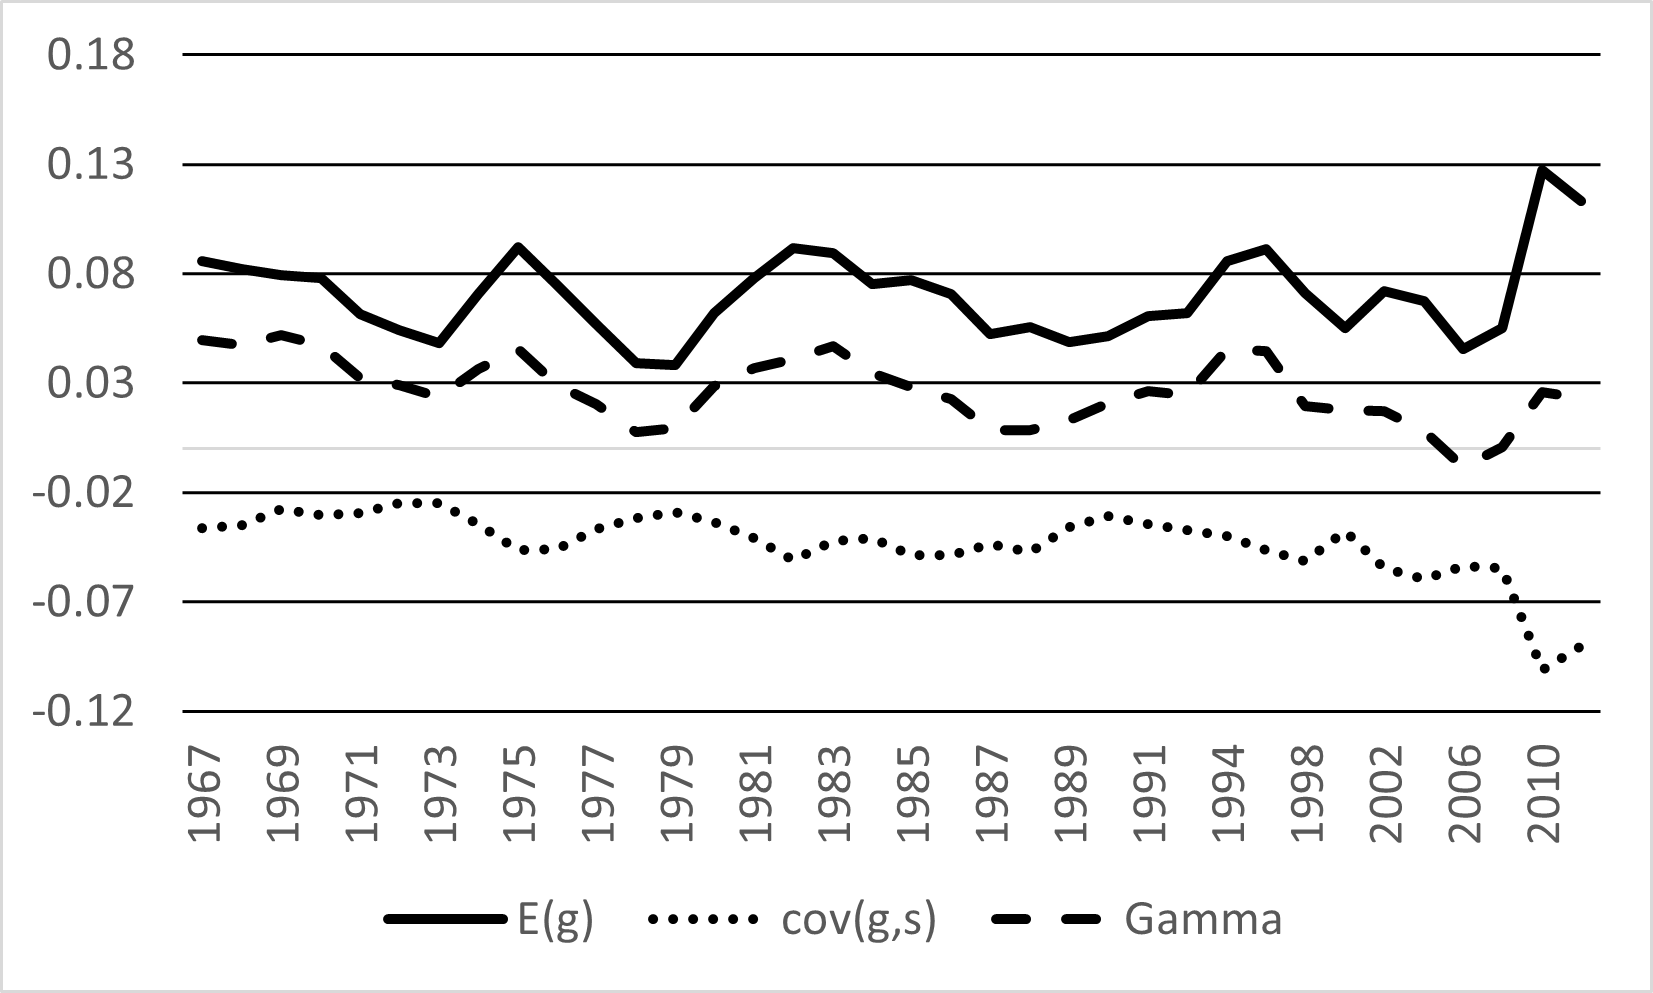
\includegraphics[width=0.48\textwidth]{Figures/Fig3_original.png}}
  \hfill
  \subfloat[Figure 4]{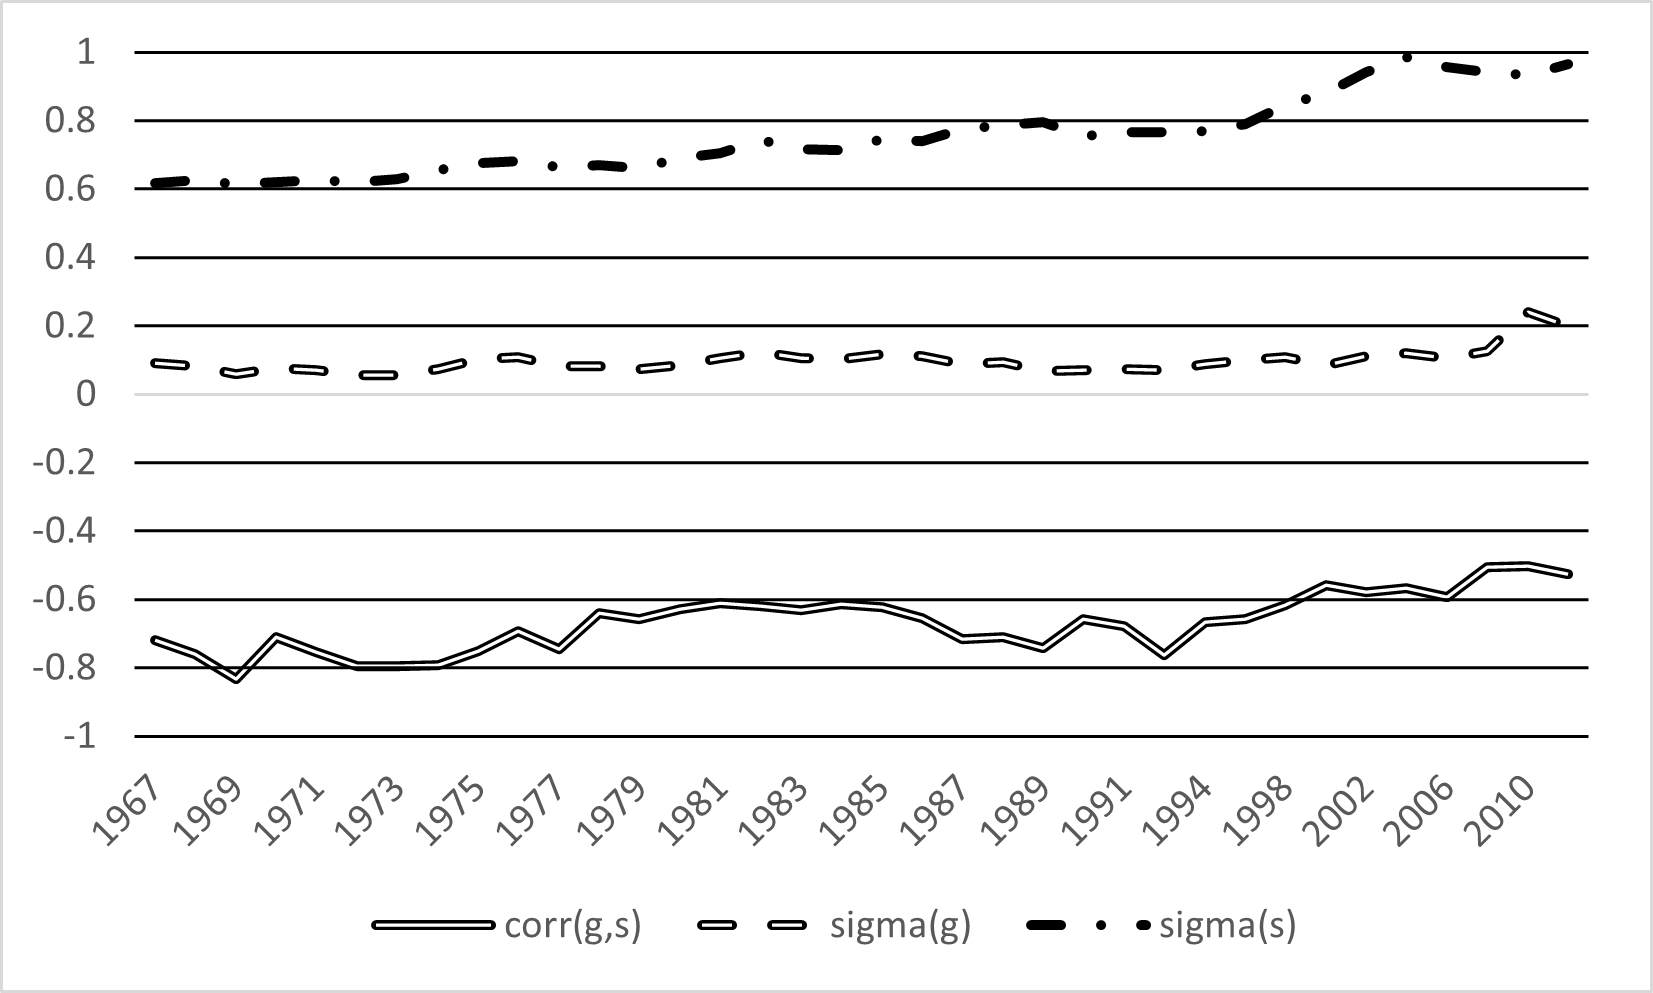
\includegraphics[width=0.48\textwidth]{Figures/Fig4_original.png}}
  \caption*{}
\end{figure}


\subsection*{Exercise 1a: exclude bottom decile}
\begin{figure}[H]
  \centering
  \subfloat[Original]{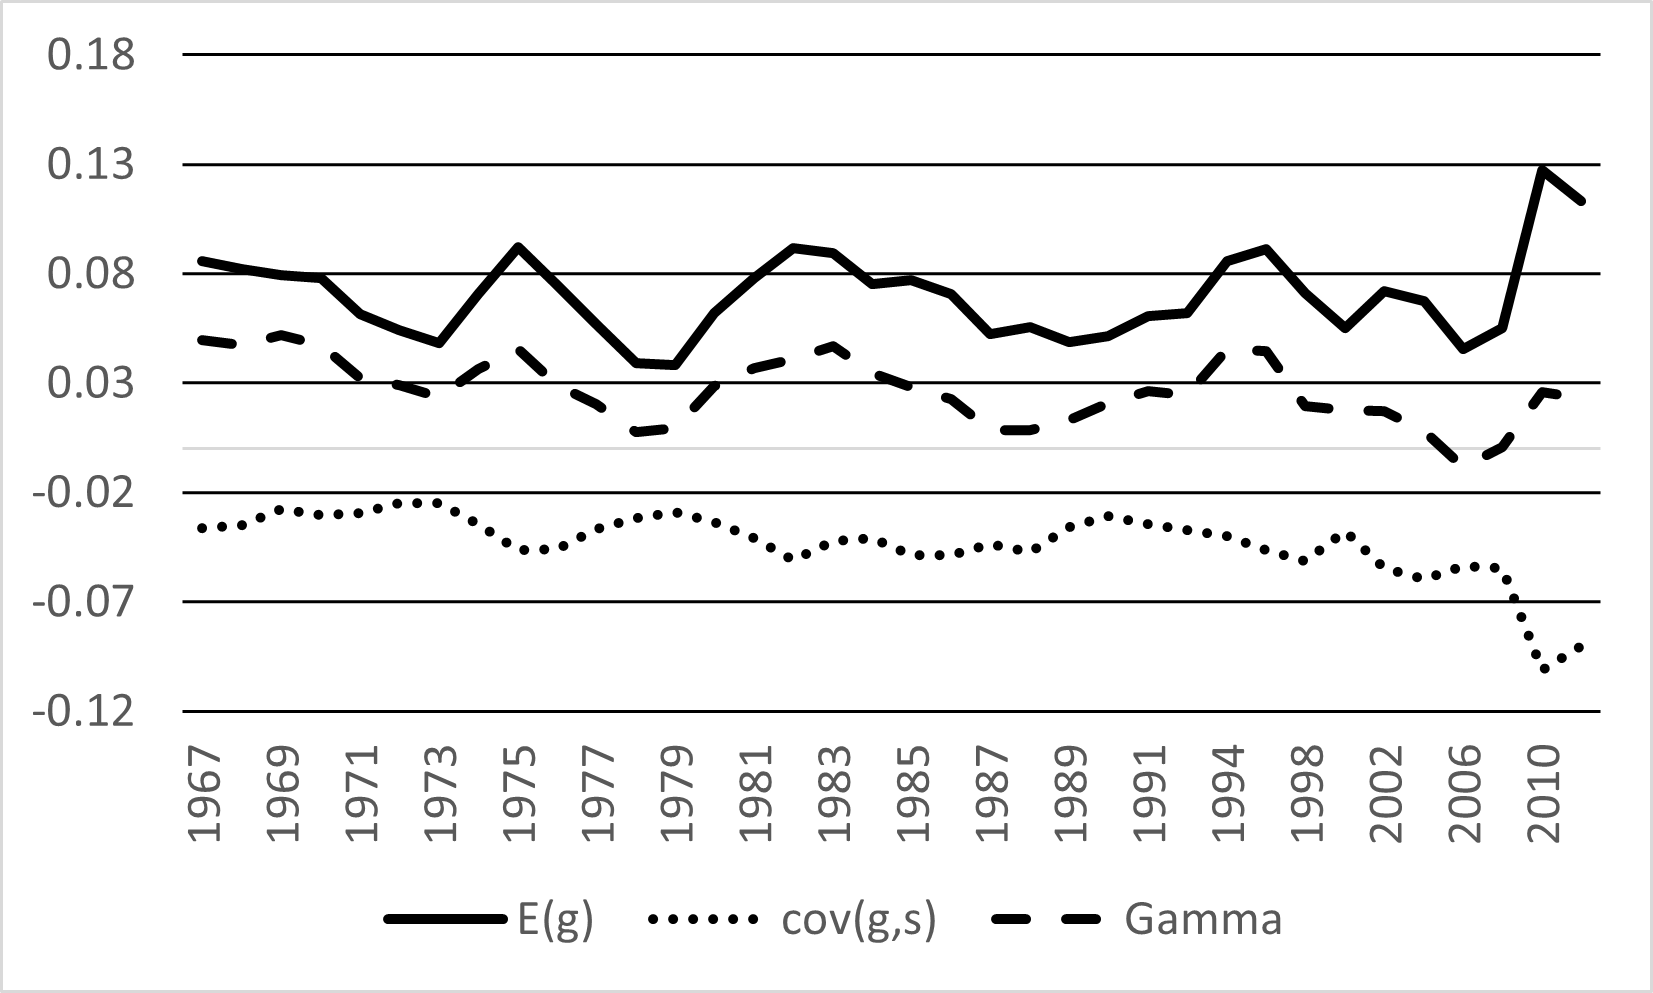
\includegraphics[width=0.48\textwidth]{Figures/Fig3_original.png}}
  \hfill
  \subfloat[No bottom decile]{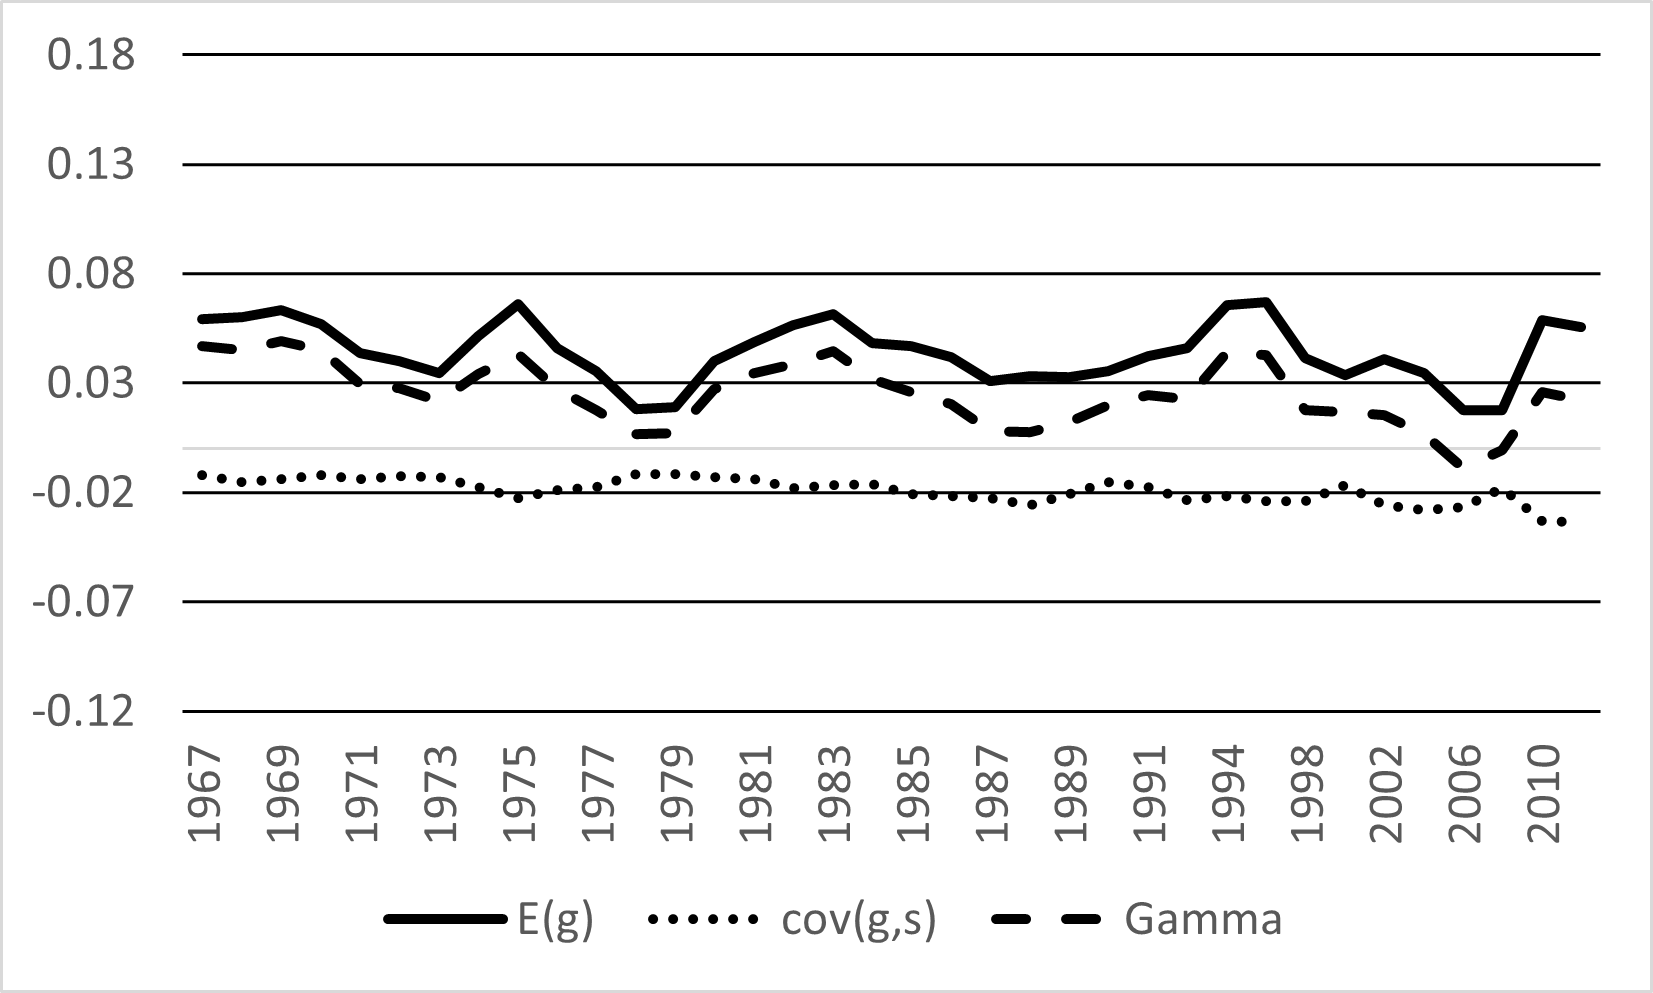
\includegraphics[width=0.48\textwidth]{Figures/Fig3_10pct.png}}
  \caption*{}
\end{figure}

There is a shift in both quantities (mean and covariance), but aggregate growth remains almost unchanged.

\begin{figure}[H]
  \centering
  \subfloat[Original]{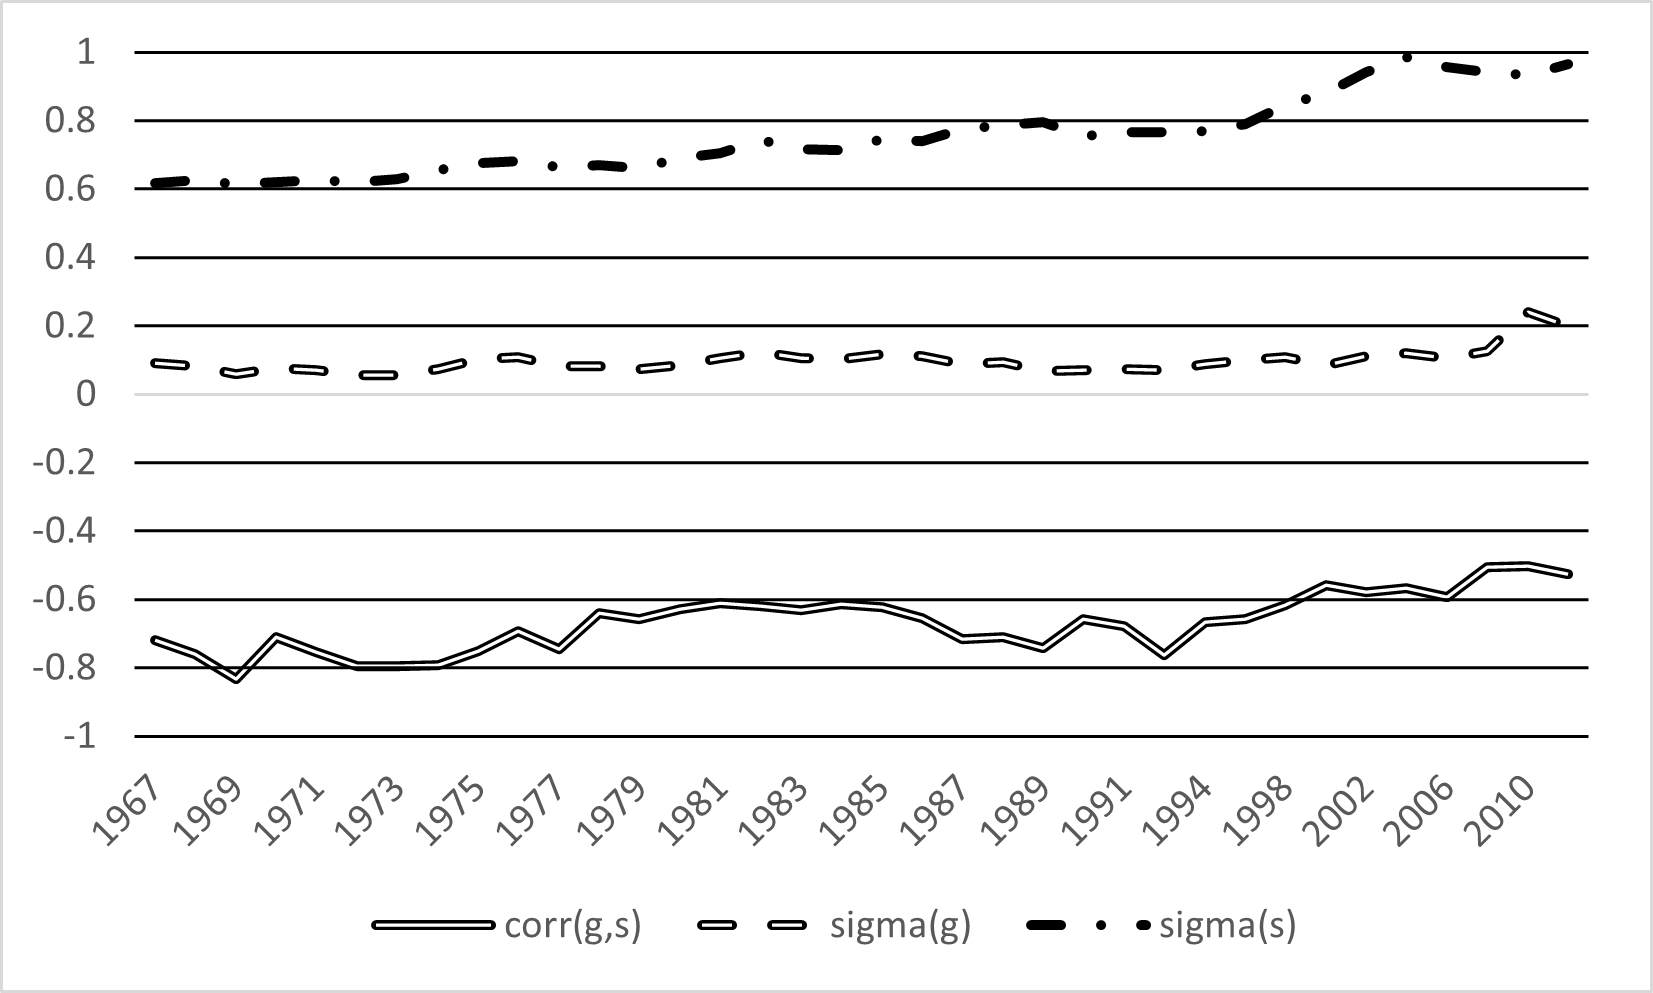
\includegraphics[width=0.48\textwidth]{Figures/Fig4_original.png}}
  \hfill
  \subfloat[No bottom decile]{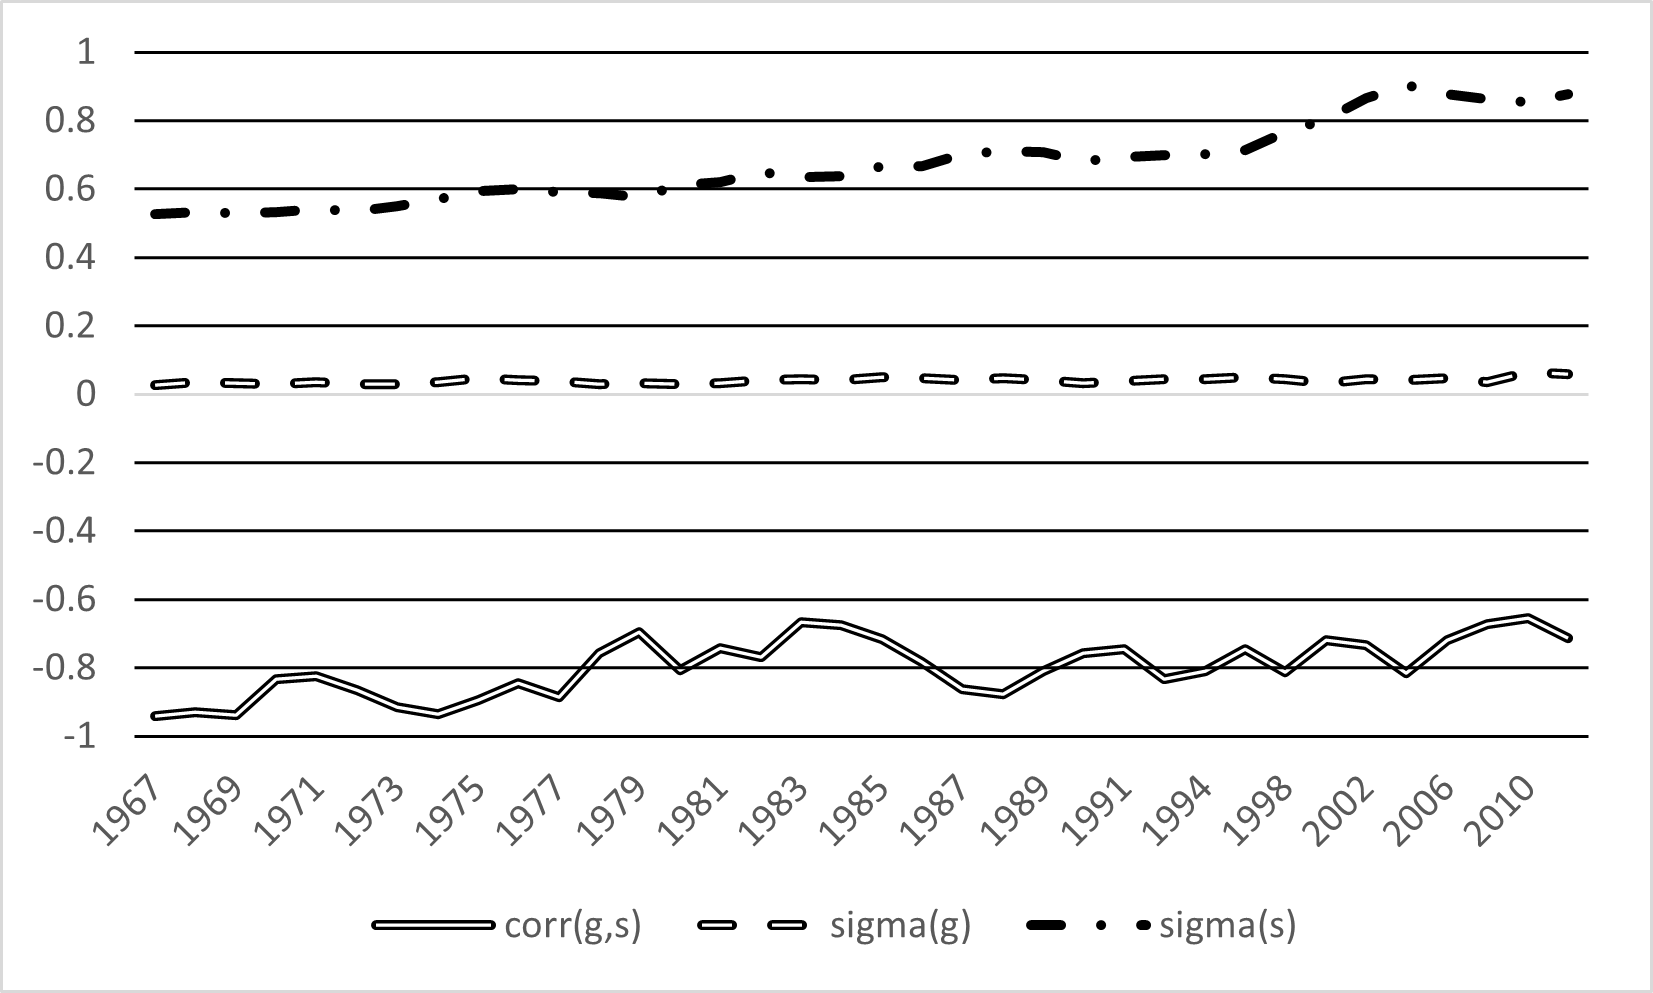
\includegraphics[width=0.48\textwidth]{Figures/Fig4_10pct.png}}
  \caption*{}
\end{figure}

\begin{itemize}
\item Since the bottom decile has the highest growth rate, by eliminating it the dispersion of growth decreases to almost zero. 
\item Inequality also decreases, as expected. 
\item The correlation is more difficult to interpret as the ``slope'' between $s$ and $g$ changes when reorganizing the top nine deciles into ten new groups (see Fig 5 of the paper).
\end{itemize}

\begin{figure}[H]
  \centering
  \subfloat[Figure 3 comparison]{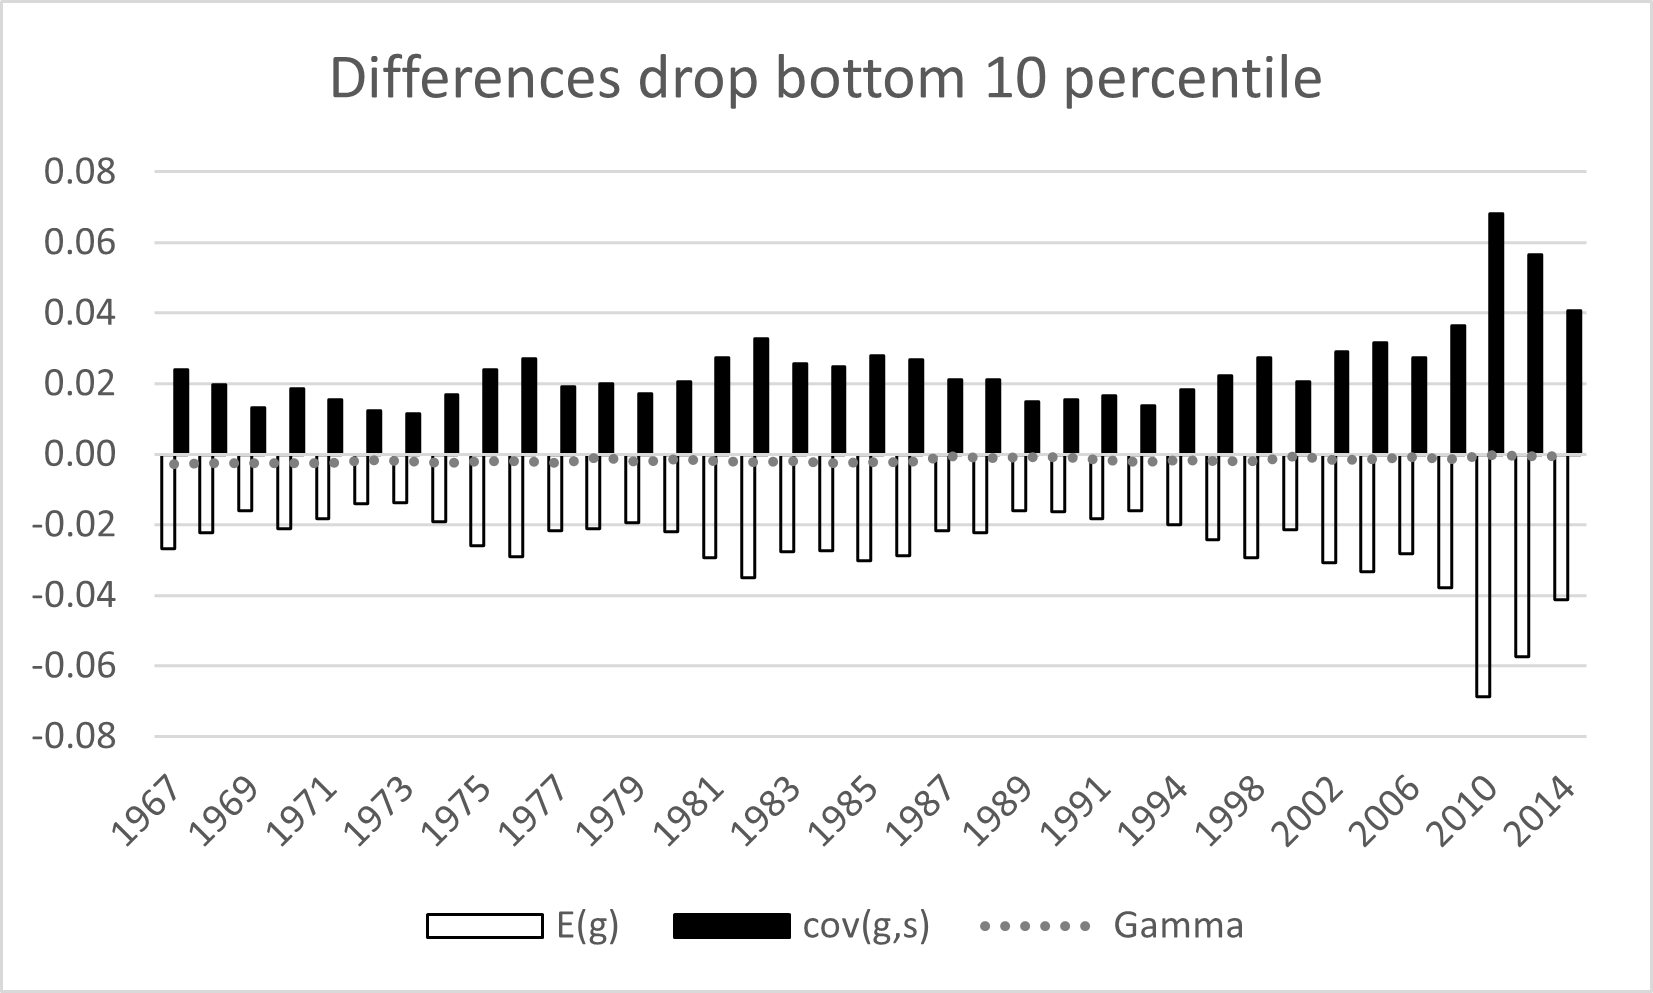
\includegraphics[width=0.48\textwidth]{Figures/Fig3_comp_10pct.png}}
  \hfill
  \subfloat[Figure 4 comparison]{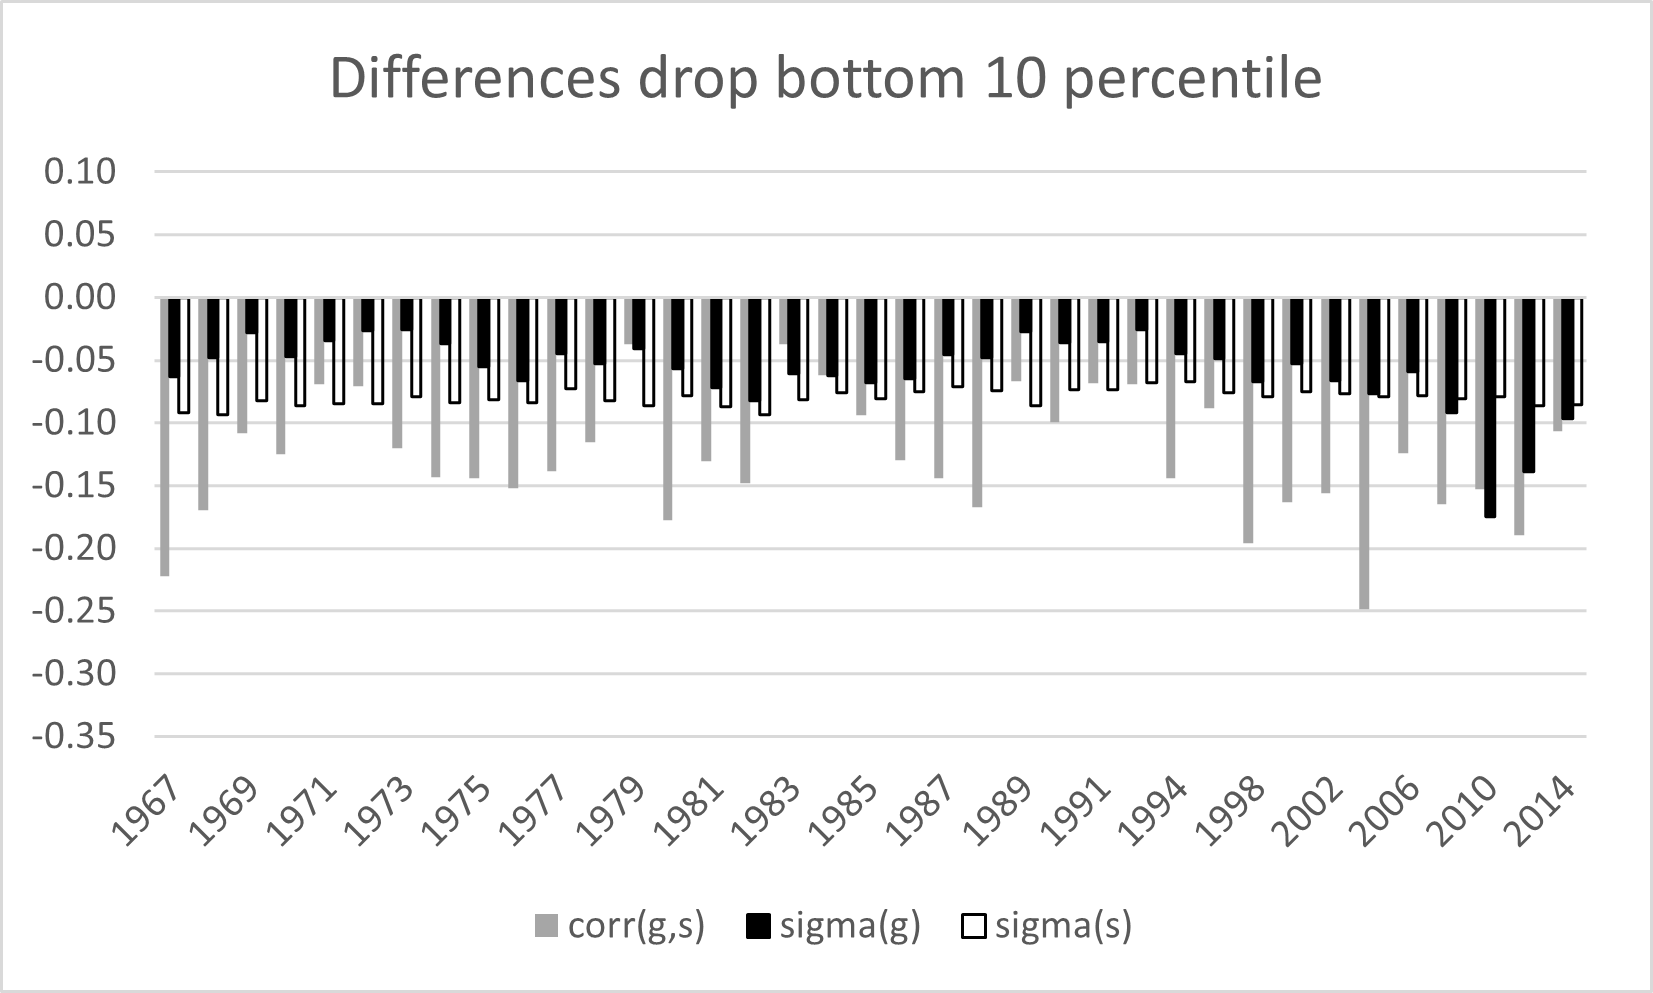
\includegraphics[width=0.48\textwidth]{Figures/Fig4_comp_10pct.png}}\\
  \subfloat[Figure 3 comparison]{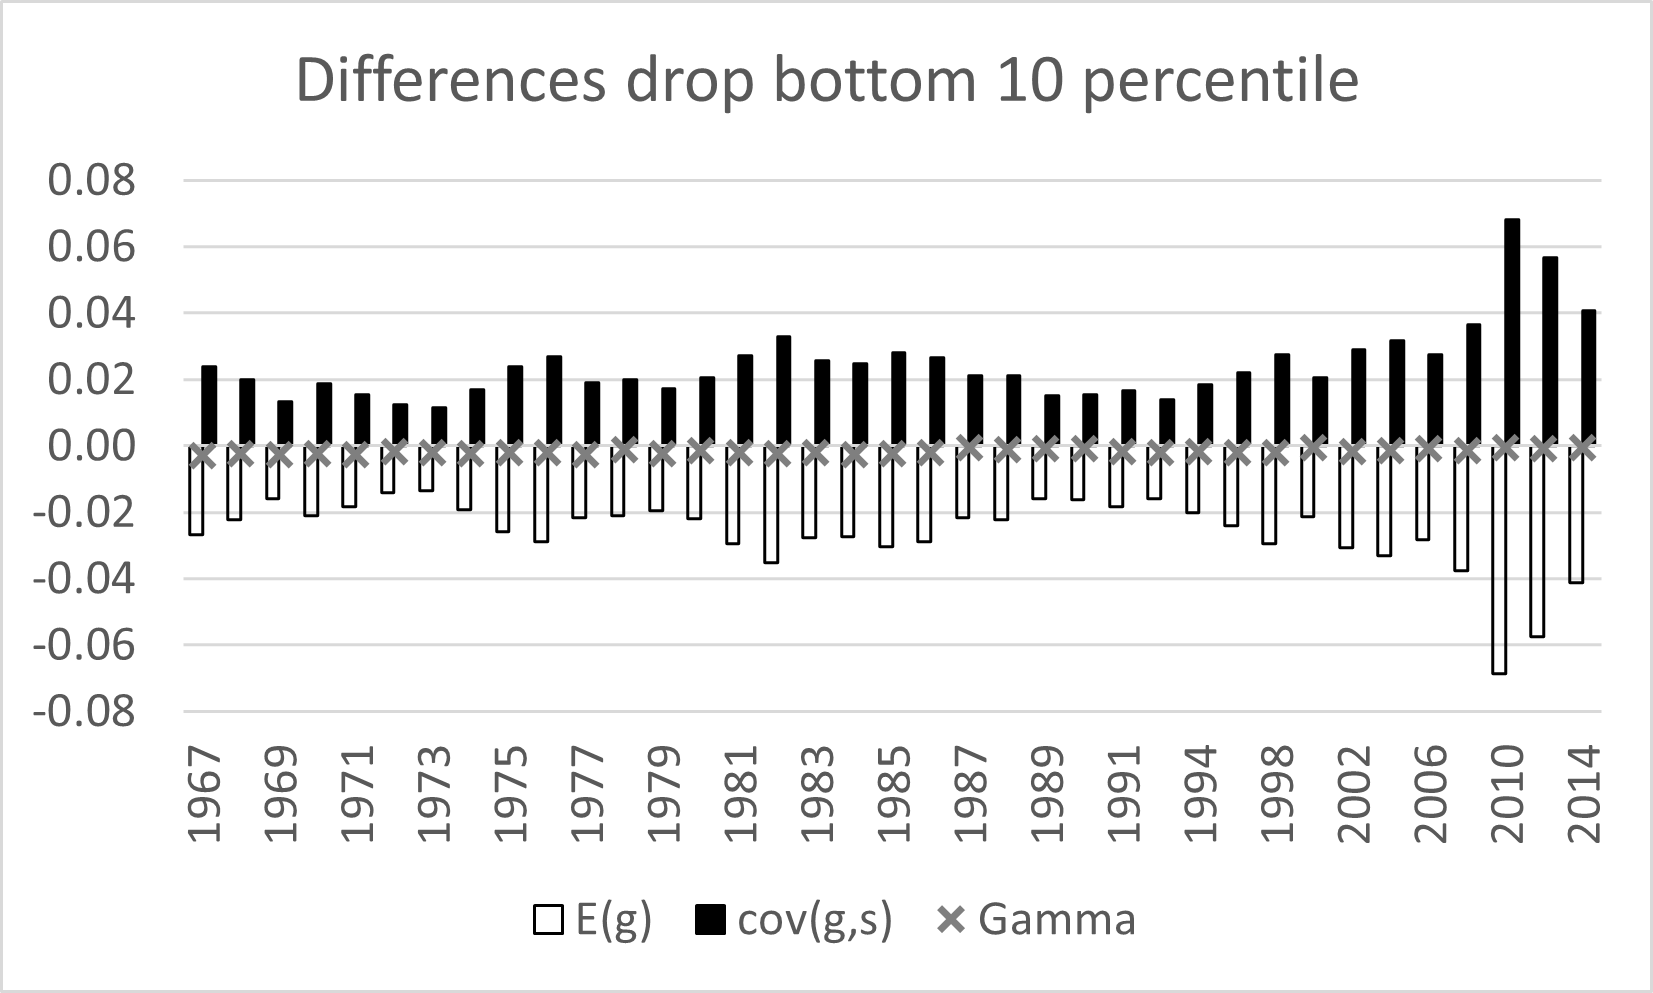
\includegraphics[width=0.48\textwidth]{Figures/Fig3_comp_10pct_optionB.png}}
  \caption*{}
\end{figure}

\begin{itemize}
    \item As pointed above, excluding the bottom decile changes a lot both the covariance and the mean, but the total effect is almost null.
    \item Both the dispersion of growth and income decreases.
    \item The correlation decreases, which means it increases in absolute value. Since the covariance increases (decreases in absolute value) this means that the decrease in volatilities dominates.
\end{itemize}

\subsection*{Exercise 1b: exclude top decile}
\begin{figure}[H]
  \centering
  \subfloat[Original]{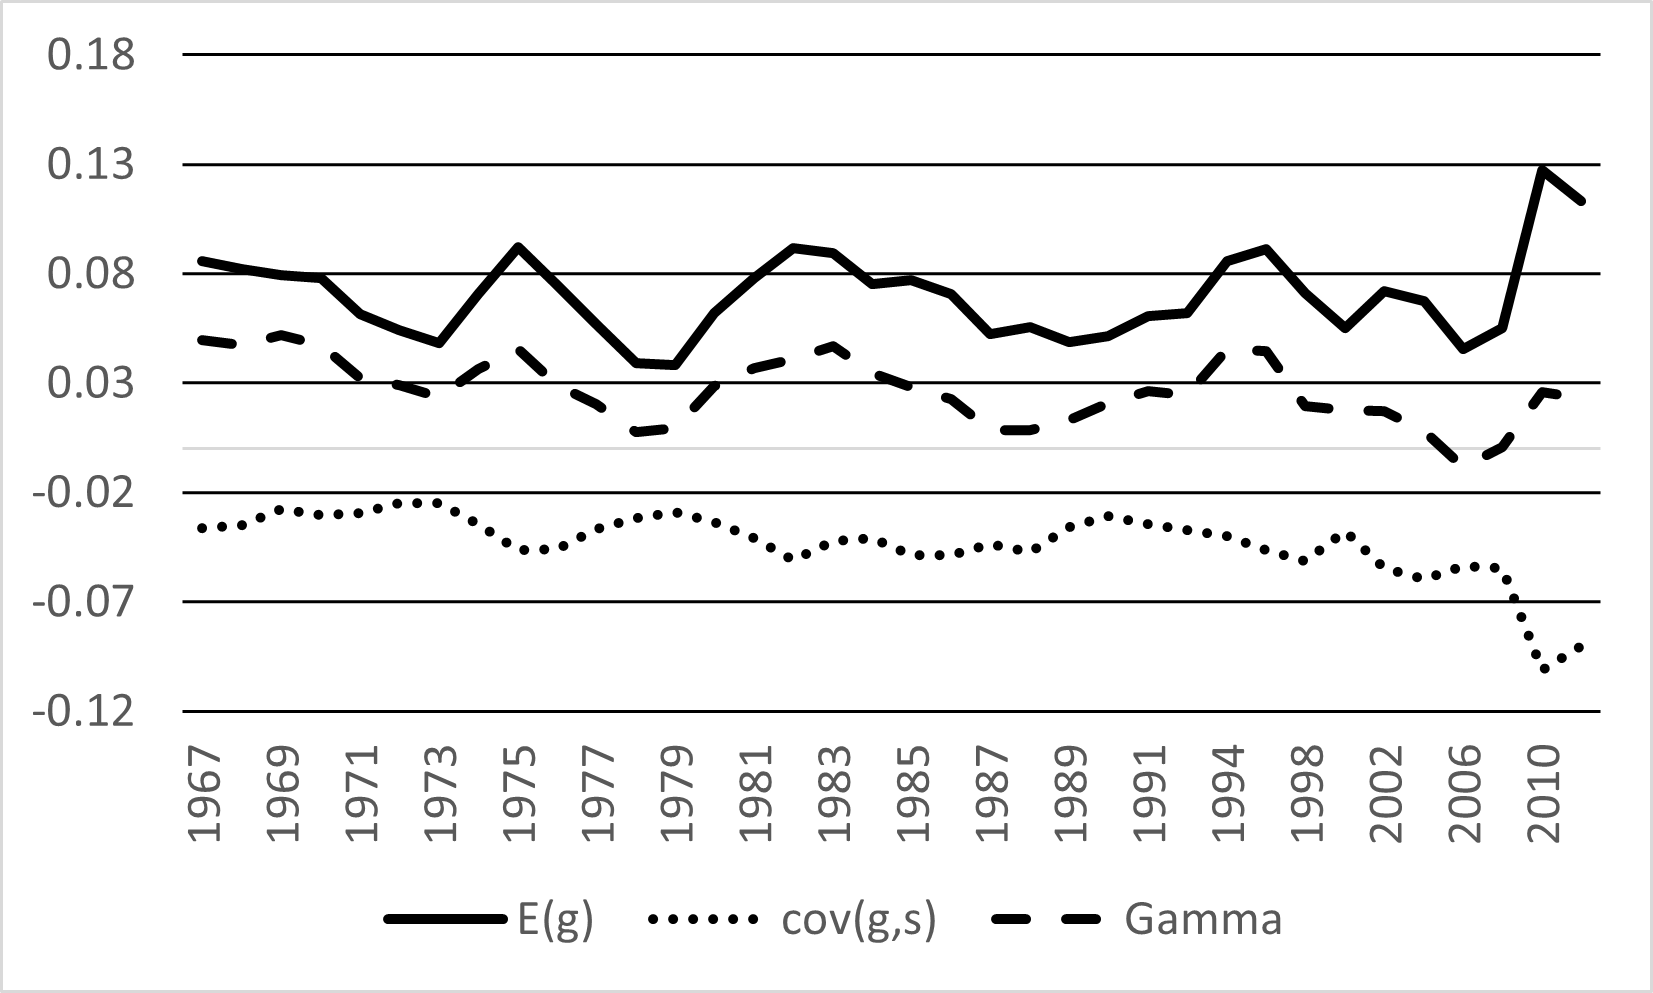
\includegraphics[width=0.48\textwidth]{Figures/Fig3_original.png}}
  \hfill
  \subfloat[No top decile]{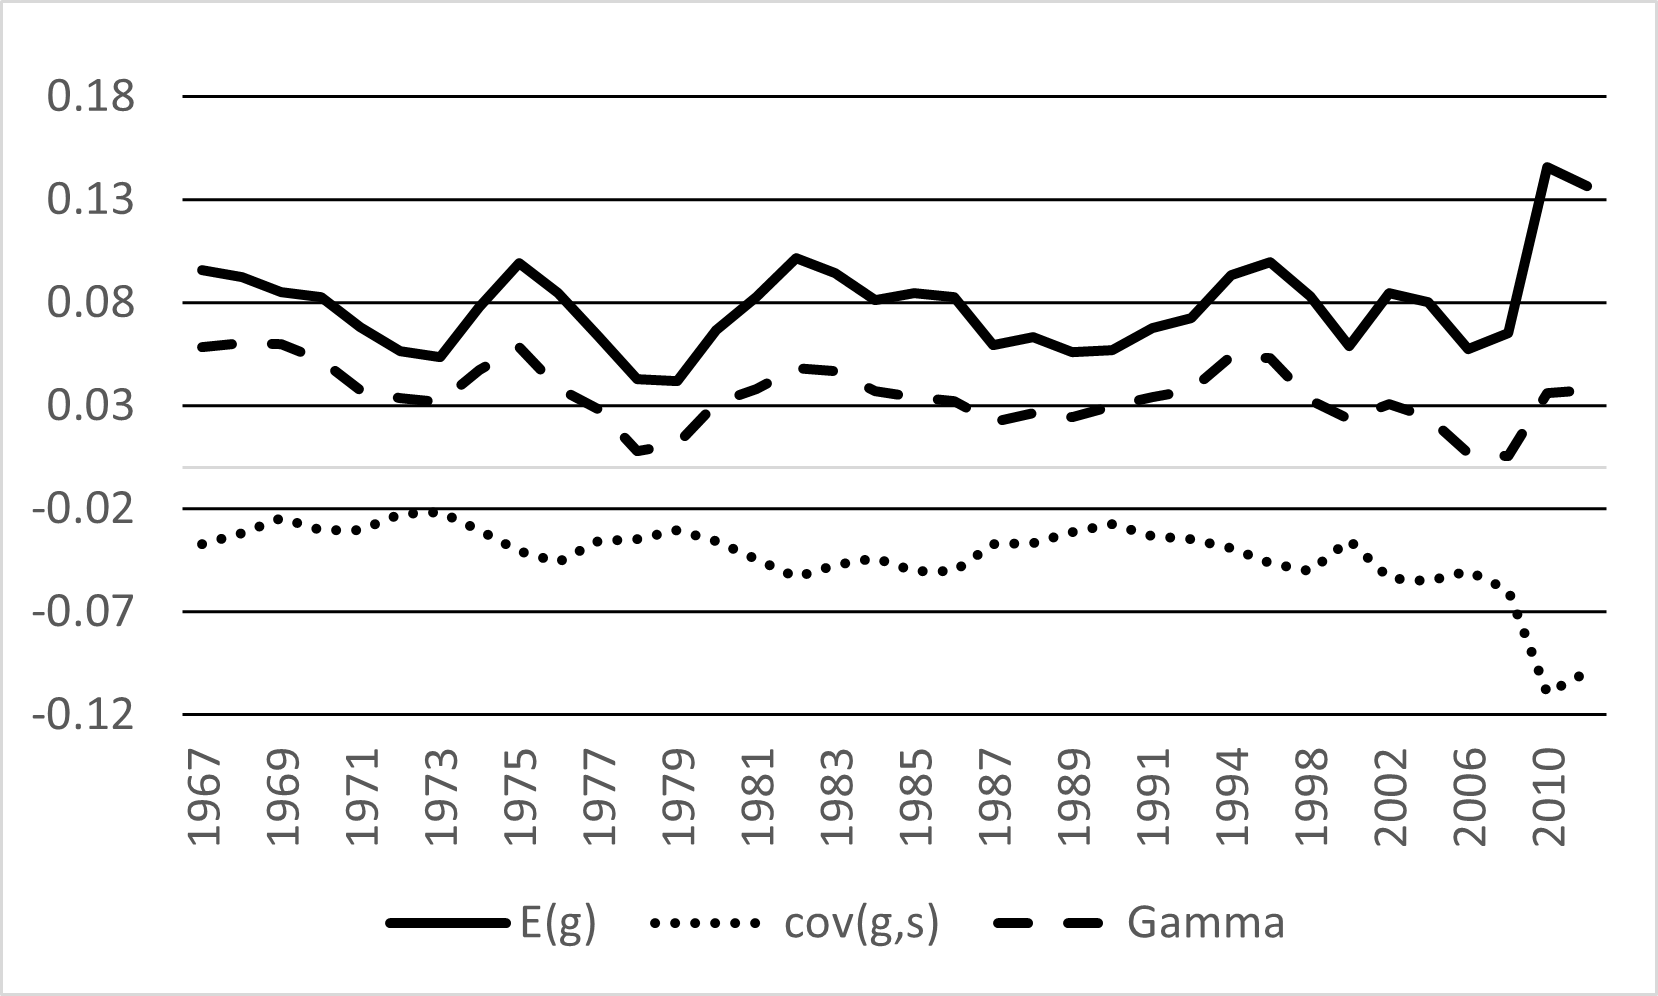
\includegraphics[width=0.48\textwidth]{Figures/Fig3_90pct.png}}
  \caption*{}
\end{figure}

\begin{itemize}
    \item Contrary to the exclusion of the bottom decile, the top decile does not change the components of aggregate growth as much.
    \item The growth dispersion remains fairly constant, unlike what happened when the bottom decile was excluded. 
    \item In this case the opposite effects of a decrease in inequality and an increase (in absolute value) of the correlation do not always have the same effect on the covariance. While in most years it was close to zero or positive by the end of the 80s, in the last years in the sample the effect on inequality dominates.
\end{itemize}

\begin{figure}[H]
  \centering
  \subfloat[Original]{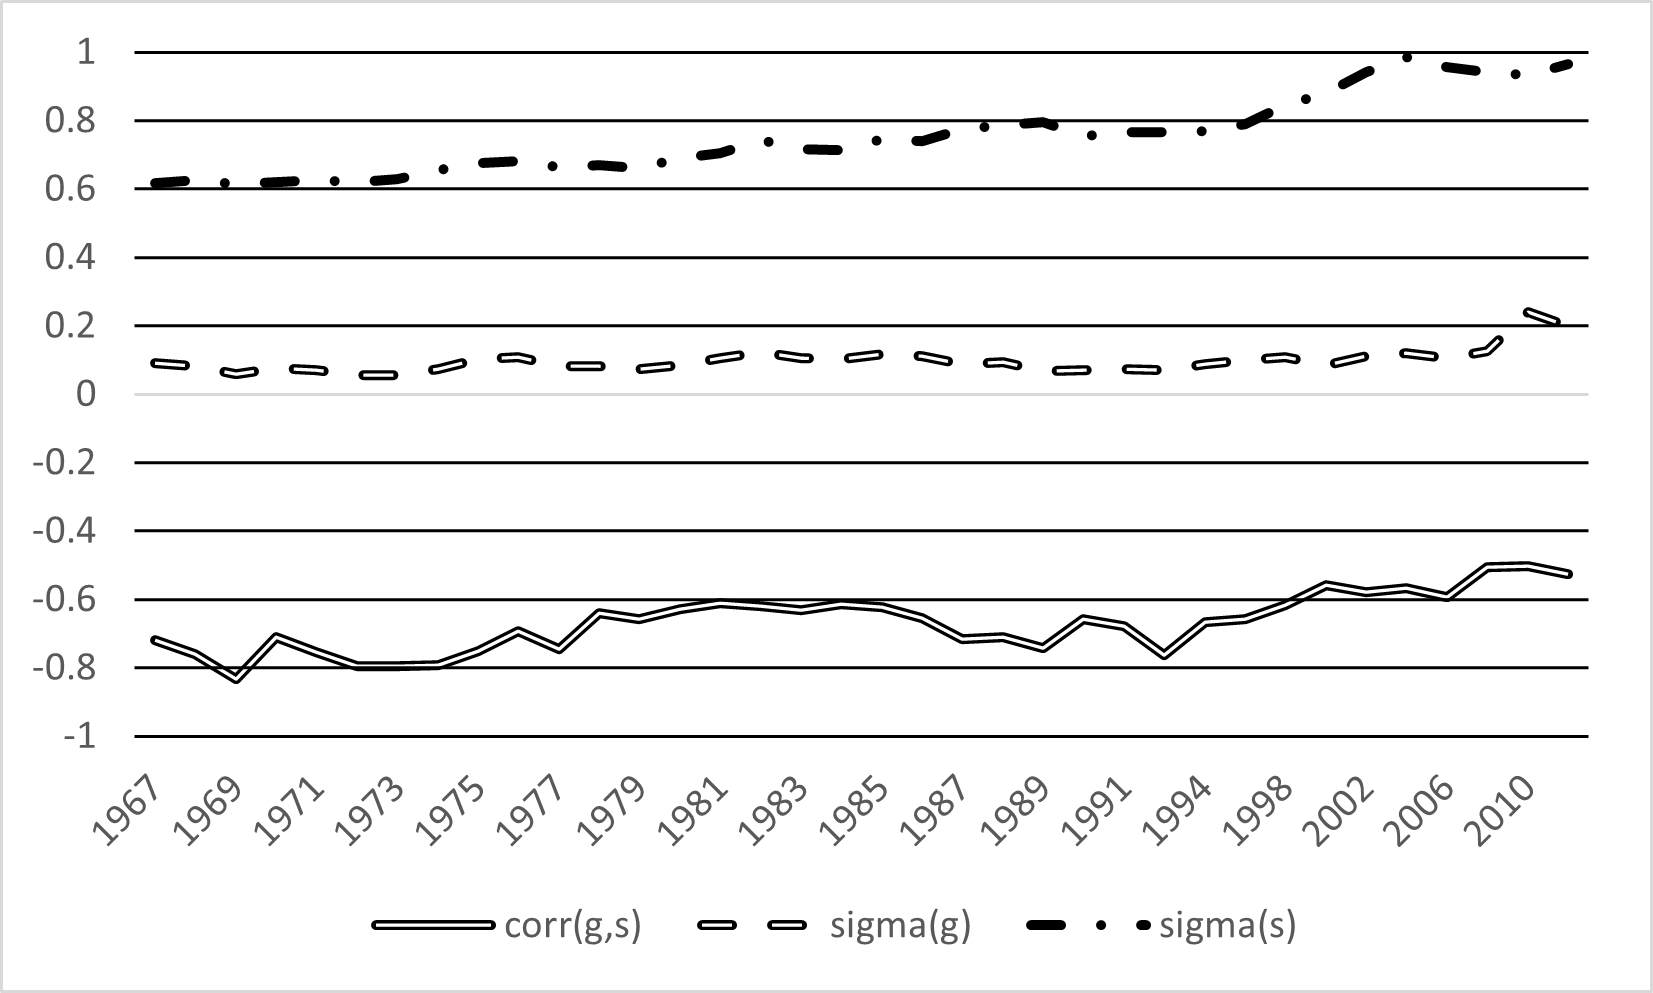
\includegraphics[width=0.48\textwidth]{Figures/Fig4_original.png}}
  \hfill
  \subfloat[No top decile]{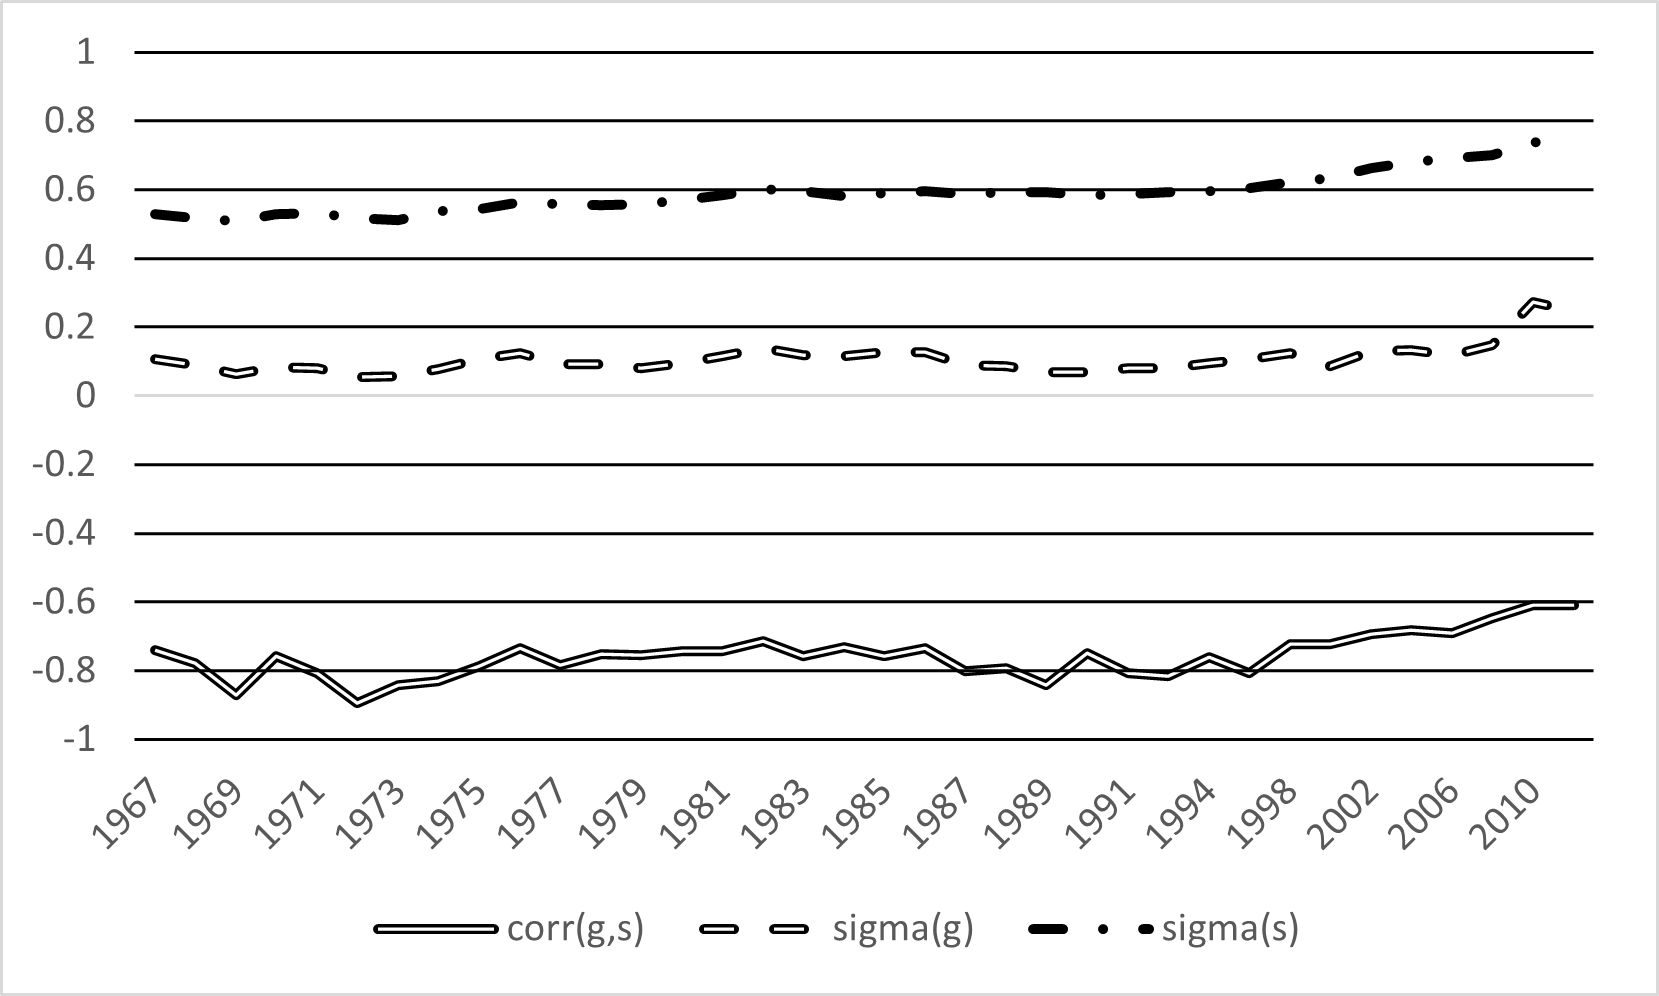
\includegraphics[width=0.48\textwidth]{Figures/Fig4_90pct.png}}
  \caption*{}
\end{figure}

\begin{itemize}
    \item There is a decrease in the correlation (increase in absolute value).
    \item There is not a big change in the volatility of growth, as it is fairly constant in the top of the income distribution.
\end{itemize}

\begin{figure}[H]
  \centering
  \subfloat[Figure 3 comparison]{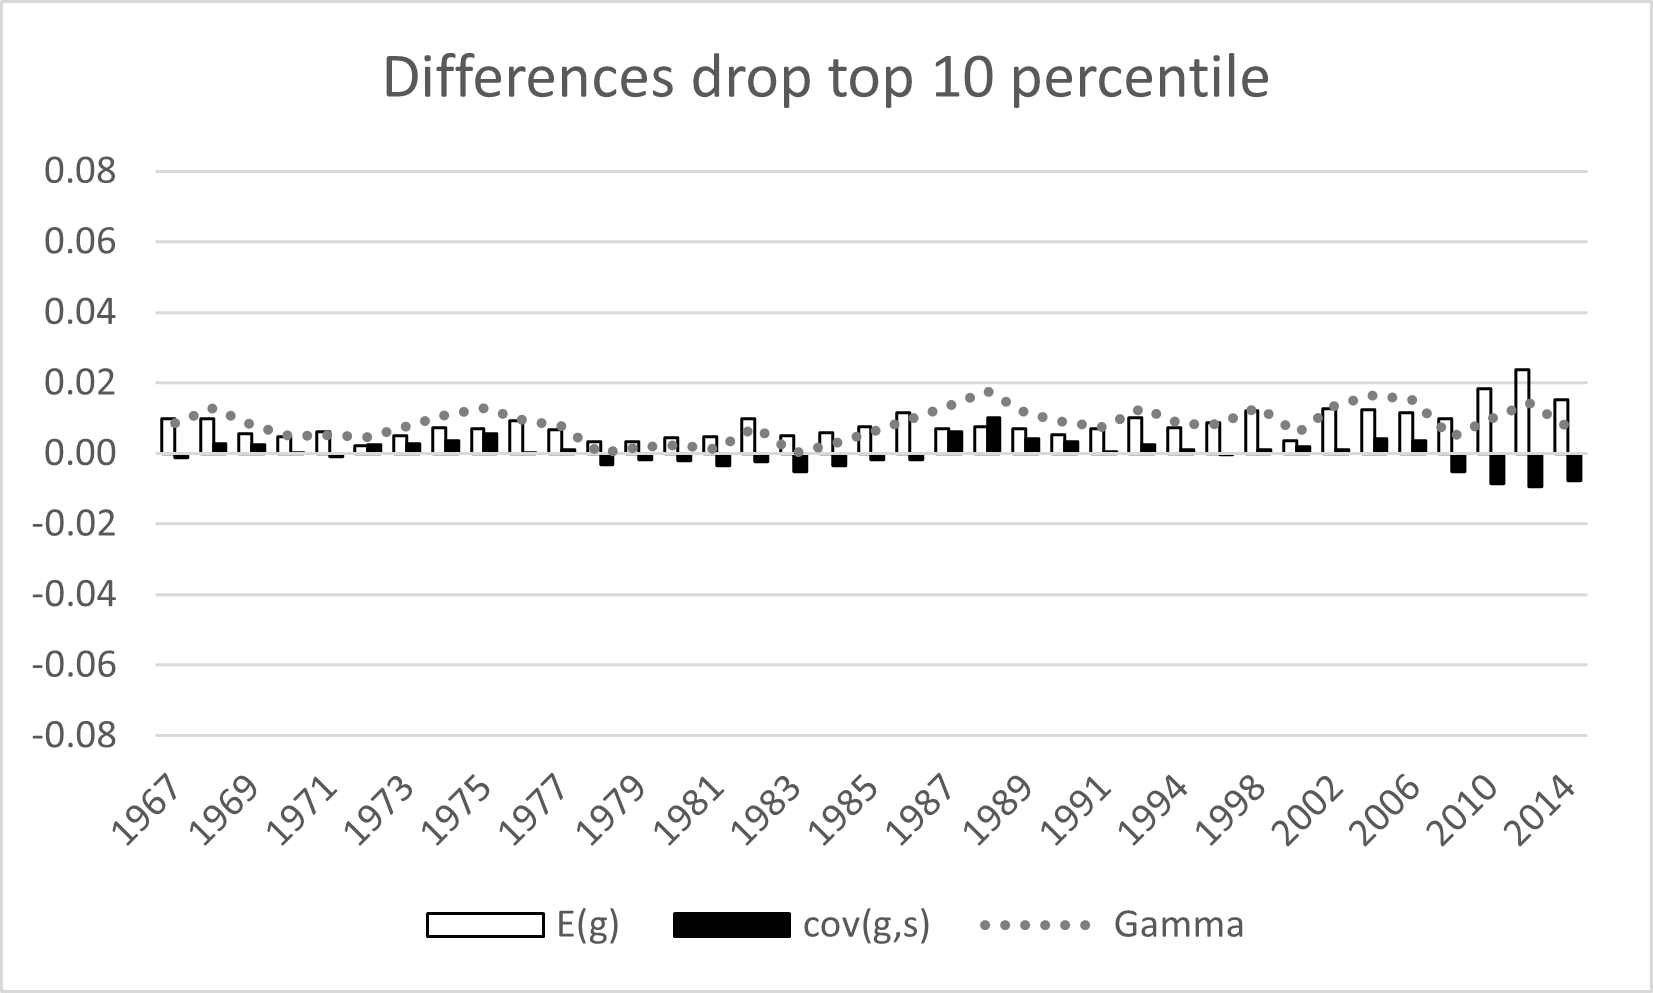
\includegraphics[width=0.48\textwidth]{Figures/Fig3_comp_90pct.png}}
  \hfill
  \subfloat[Figure 4 comparison]{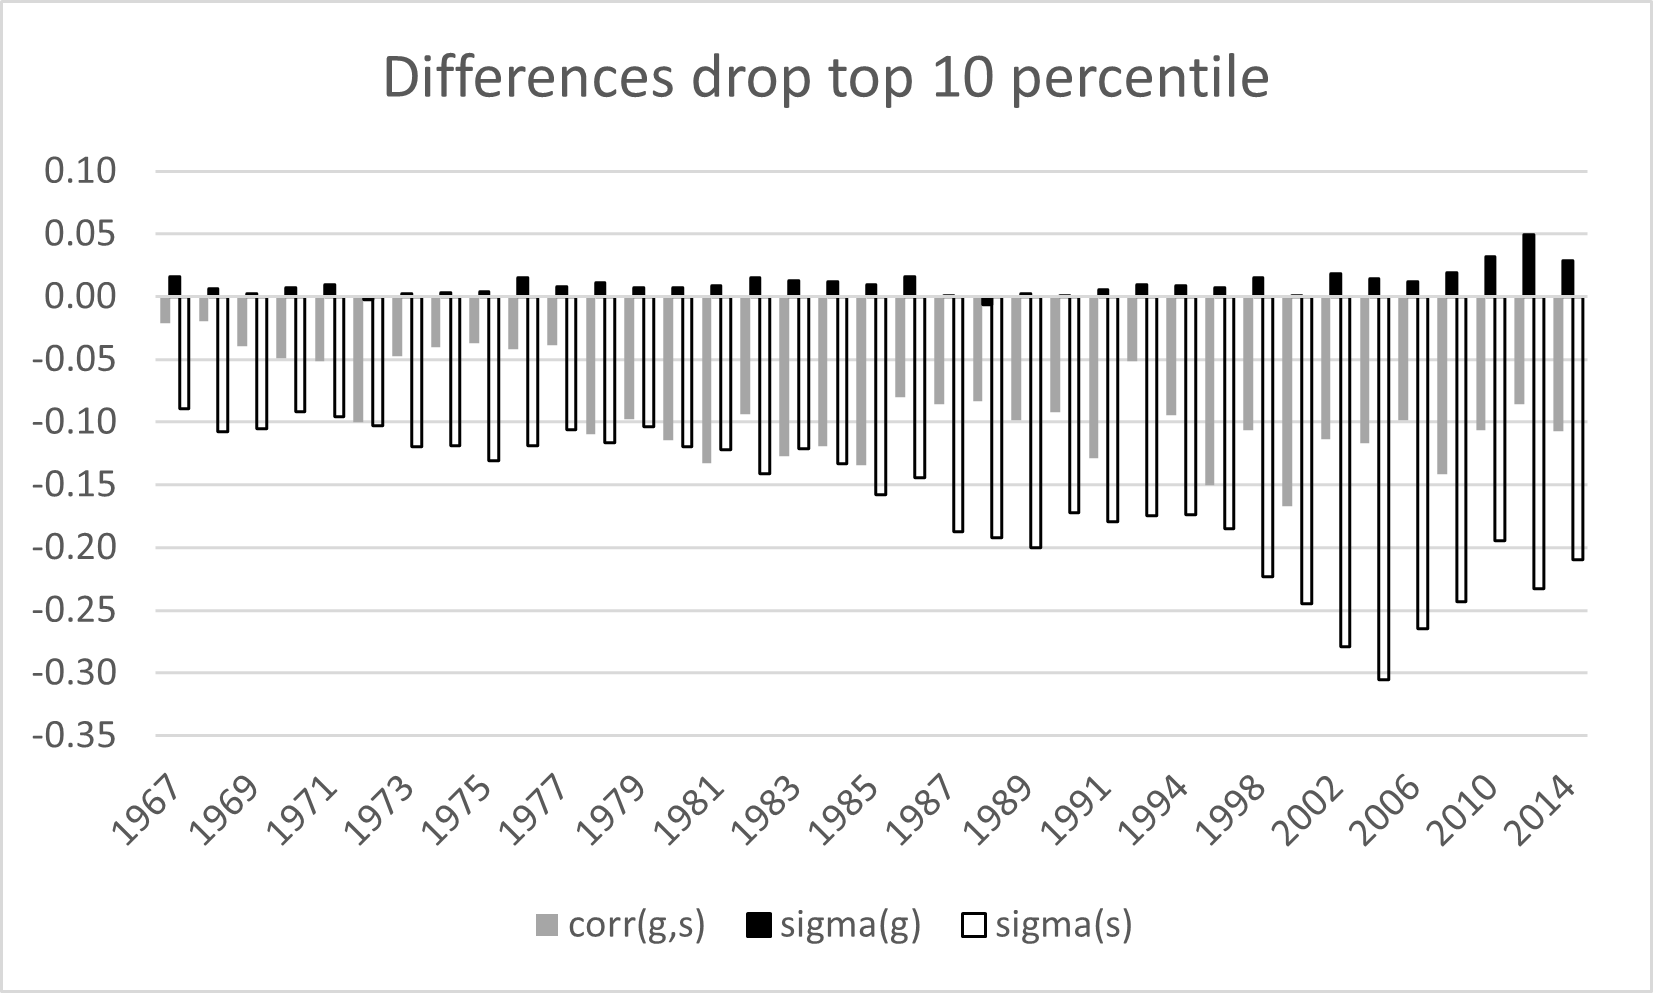
\includegraphics[width=0.48\textwidth]{Figures/Fig4_comp_90pct.png}}\\
  \subfloat[Figure 3 comparison]{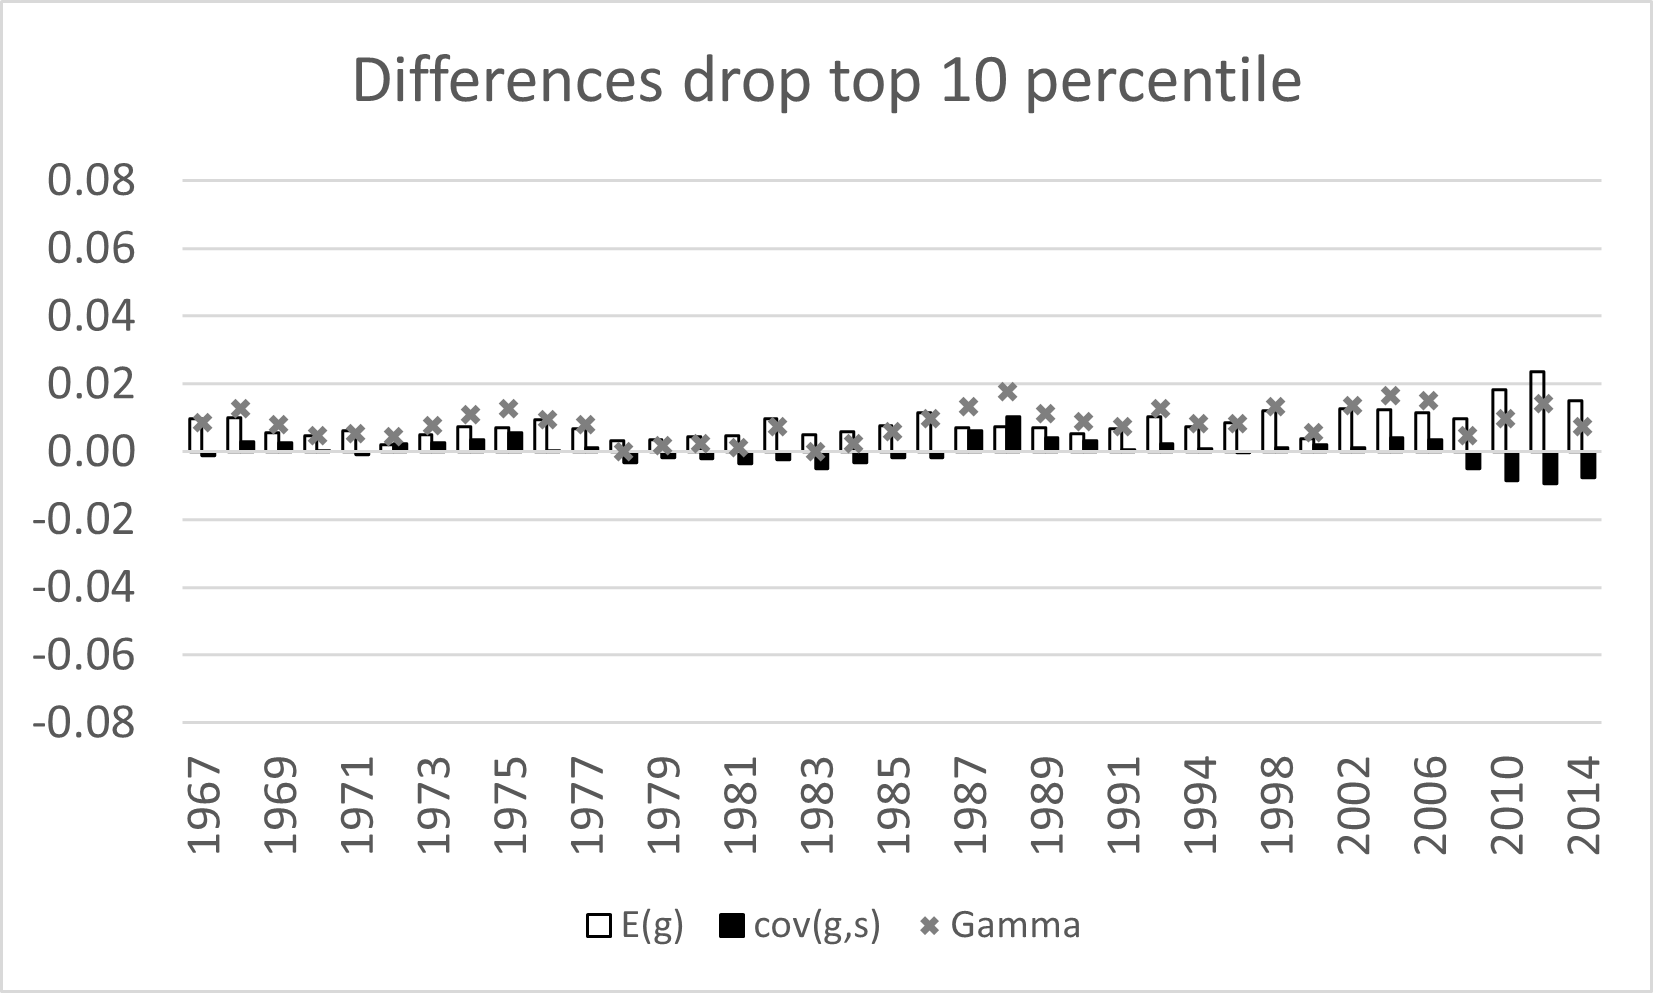
\includegraphics[width=0.48\textwidth]{Figures/Fig3_comp_90pct_optionB.png}}
  \caption*{}
\end{figure}

\begin{itemize}
    \item The changes in the components of total growth is not as much as with the exclusion of the bottom decile. However, the effect on total growth is higher in this case.
    \item Inequality decreases.
    \item Growth dispersion is not changed as much, since the growth for the top decile is not that different from other deciles on the top of the distribution.
    \item The correlation decreases (increases in absolute value), implying that the slope between growth and income is steeper.
\end{itemize}


\subsection*{Exercise 1c: comparison of growth}

\begin{figure}[H]
  \centering
  \subfloat[Values]{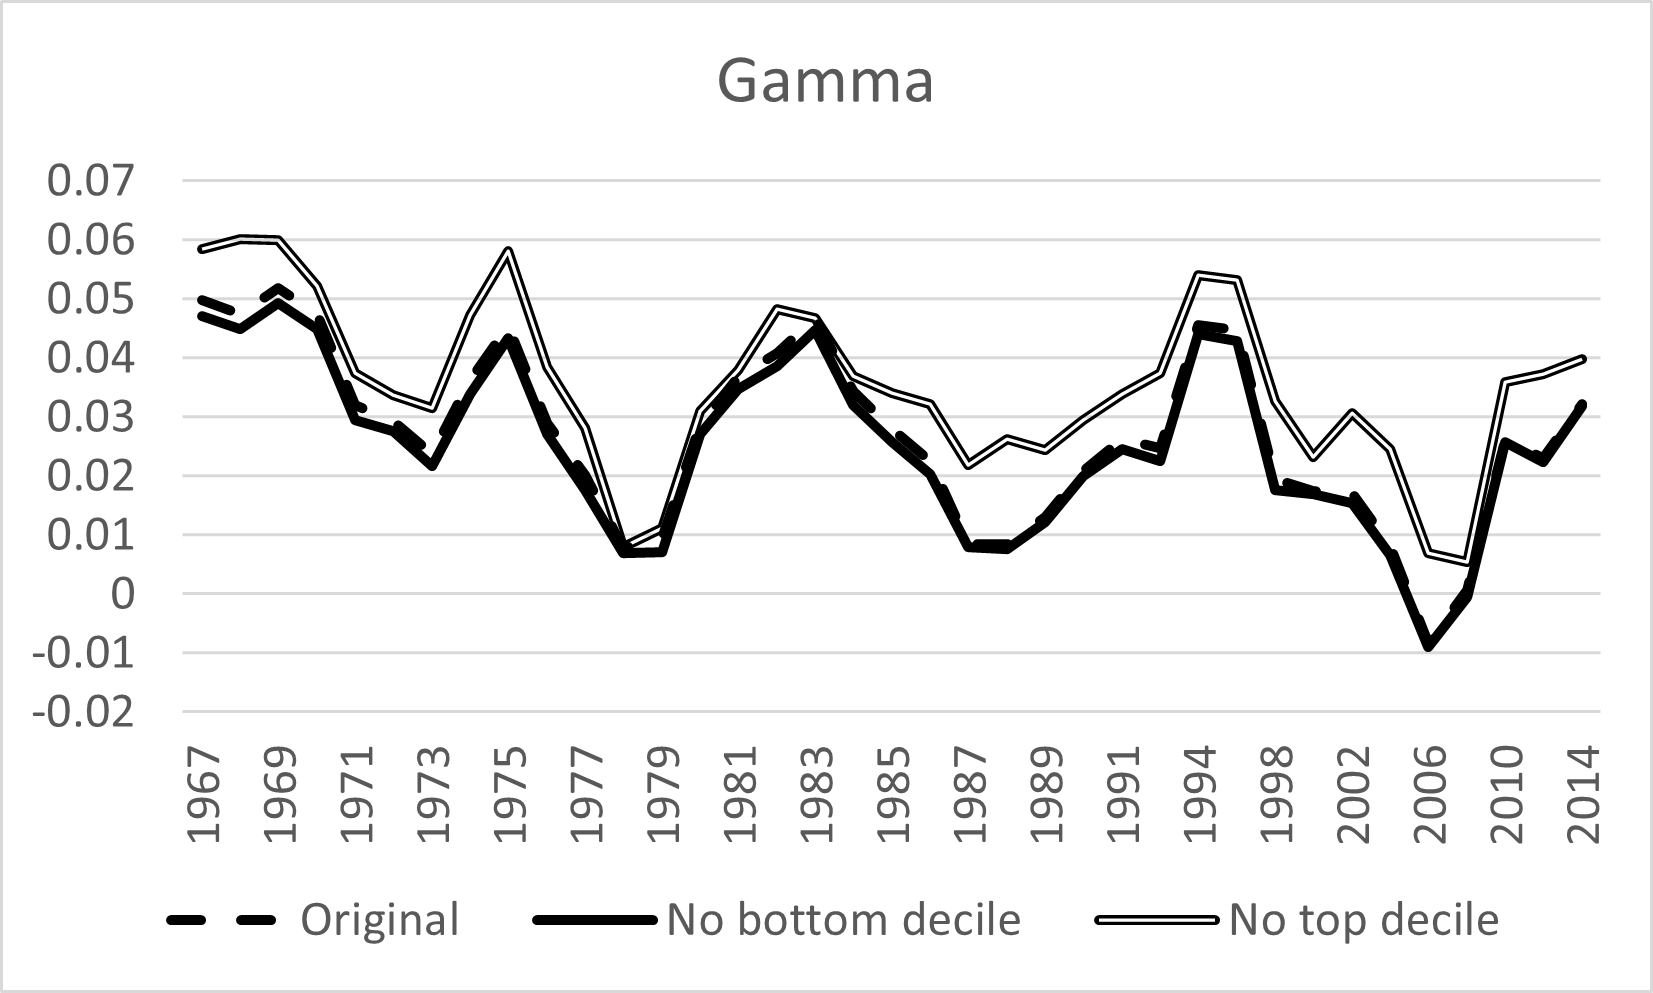
\includegraphics[width=0.48\textwidth]{Figures/Gamma_comparison_deciles.png}}
  \hfill
  \subfloat[Differences]{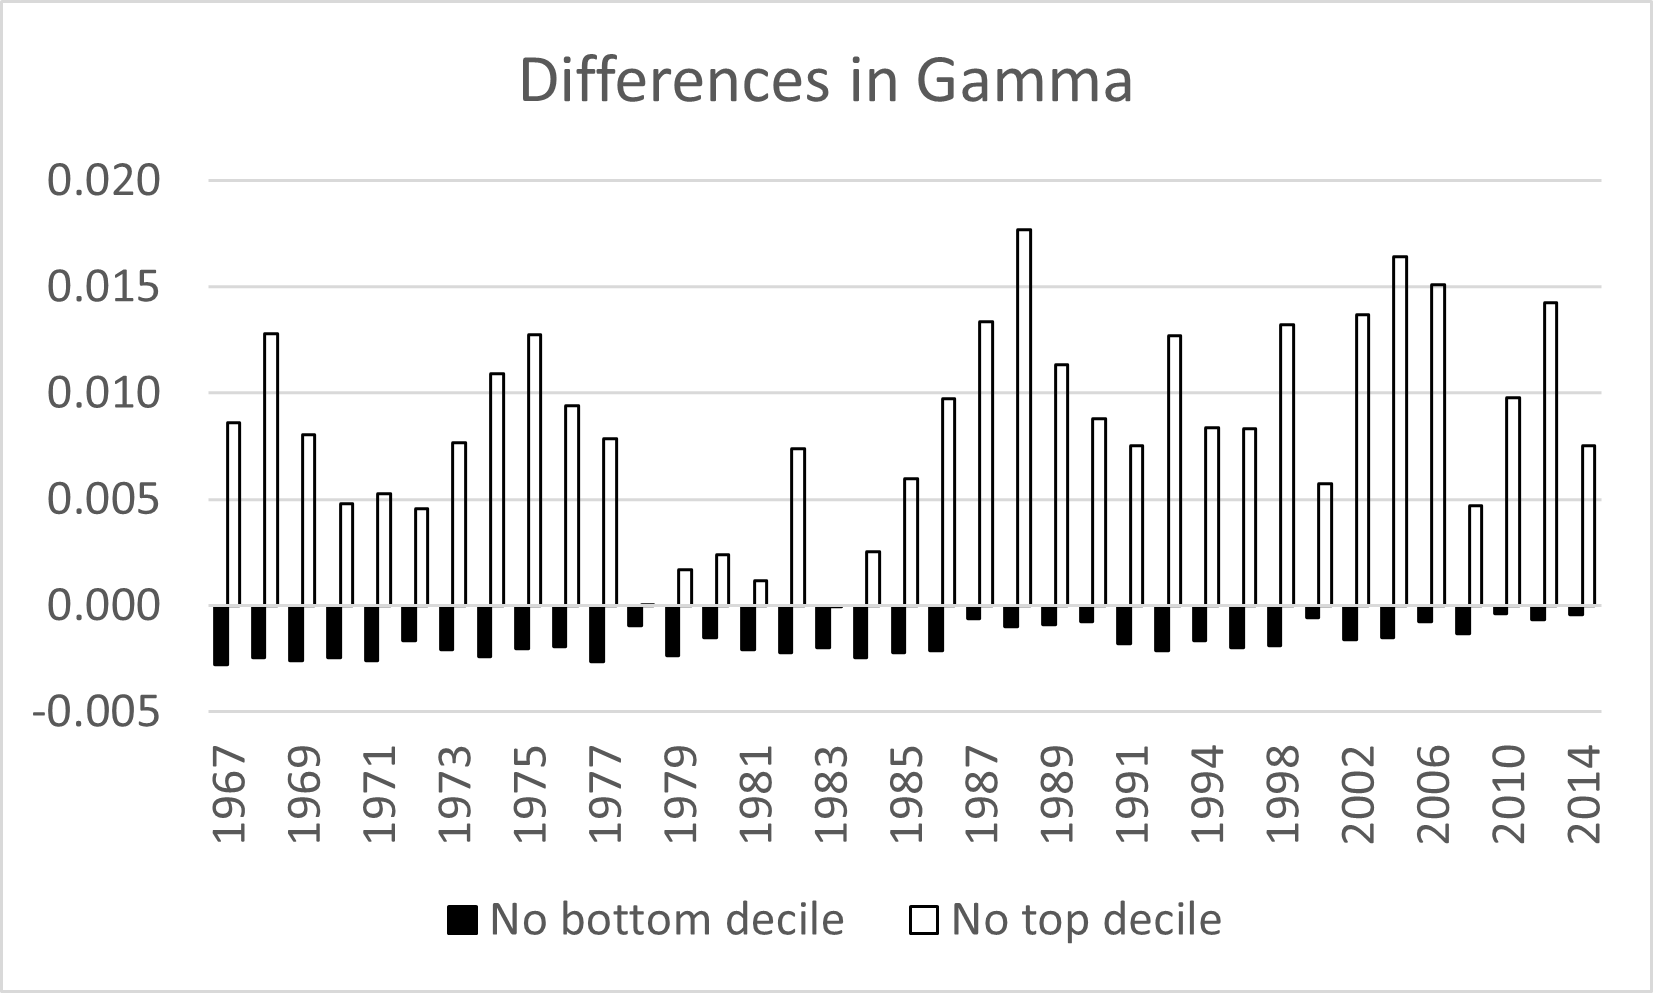
\includegraphics[width=0.48\textwidth]{Figures/Gamma_differences_deciles.png}}
  \caption*{}
\end{figure}

\begin{itemize}
    \item The effect of the top decile is higher on total growth than the one of the bottom decile.
\end{itemize}

\subsection*{Exercise 2: keep correlation or standard deviations constant}

\begin{figure}[H]
  \centering
  \subfloat[Values]{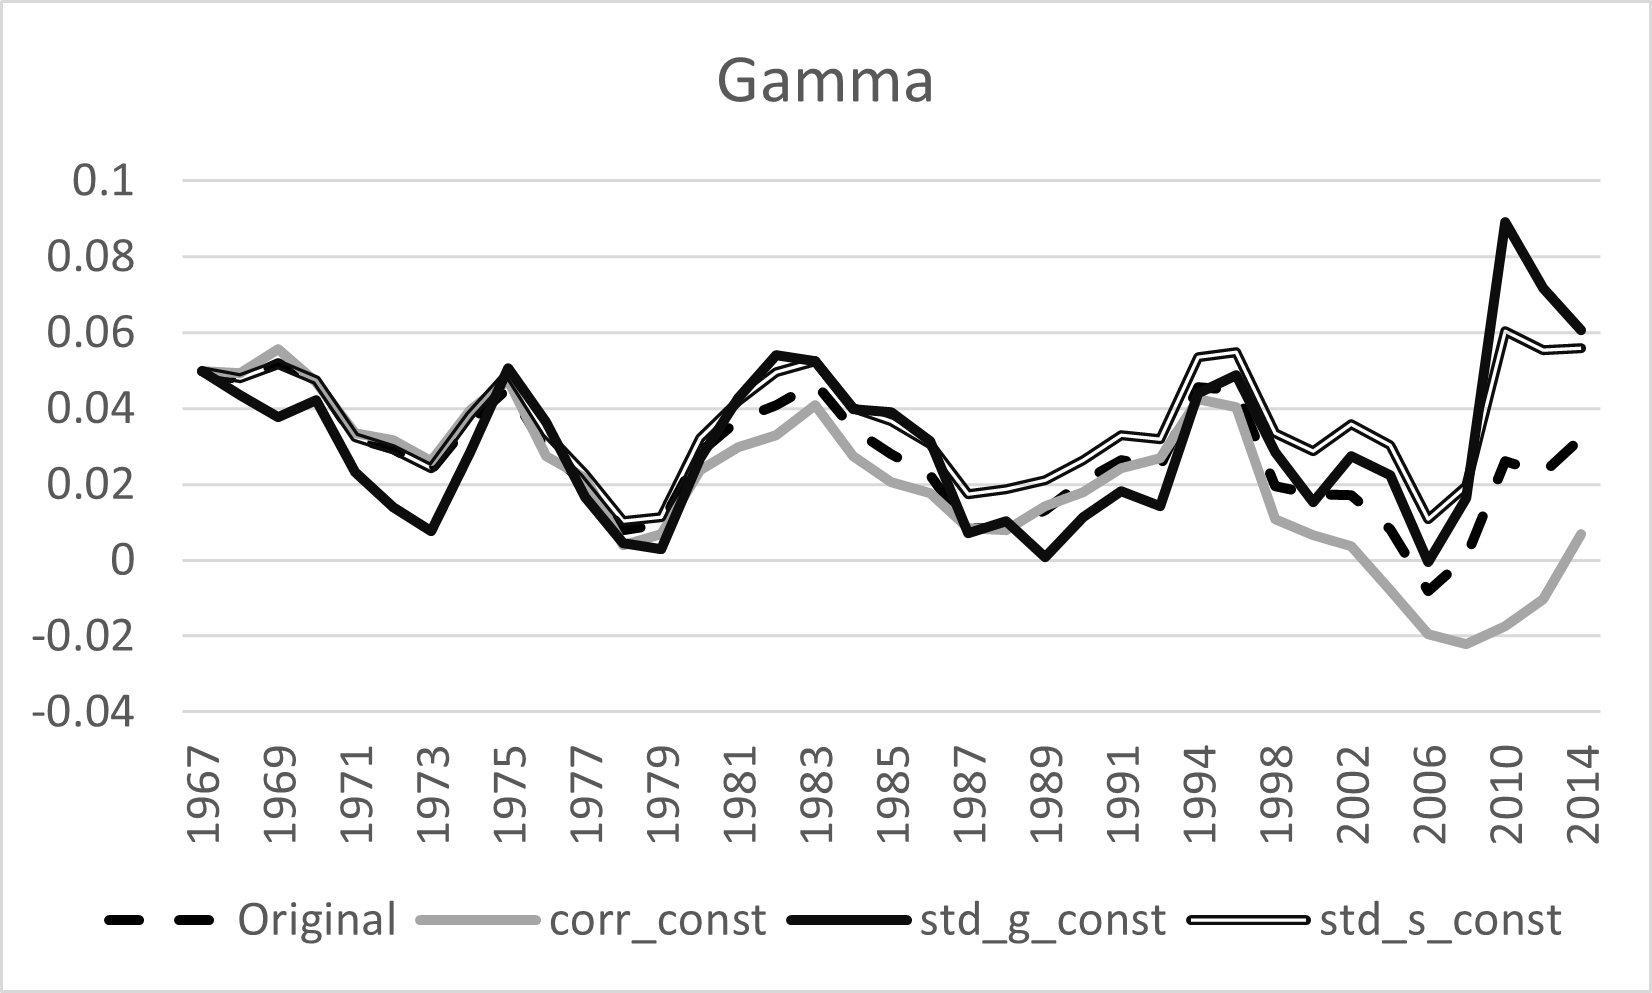
\includegraphics[width=0.48\textwidth]{Figures/Gamma_comparisons.png}}
  \hfill
  \subfloat[Differences]{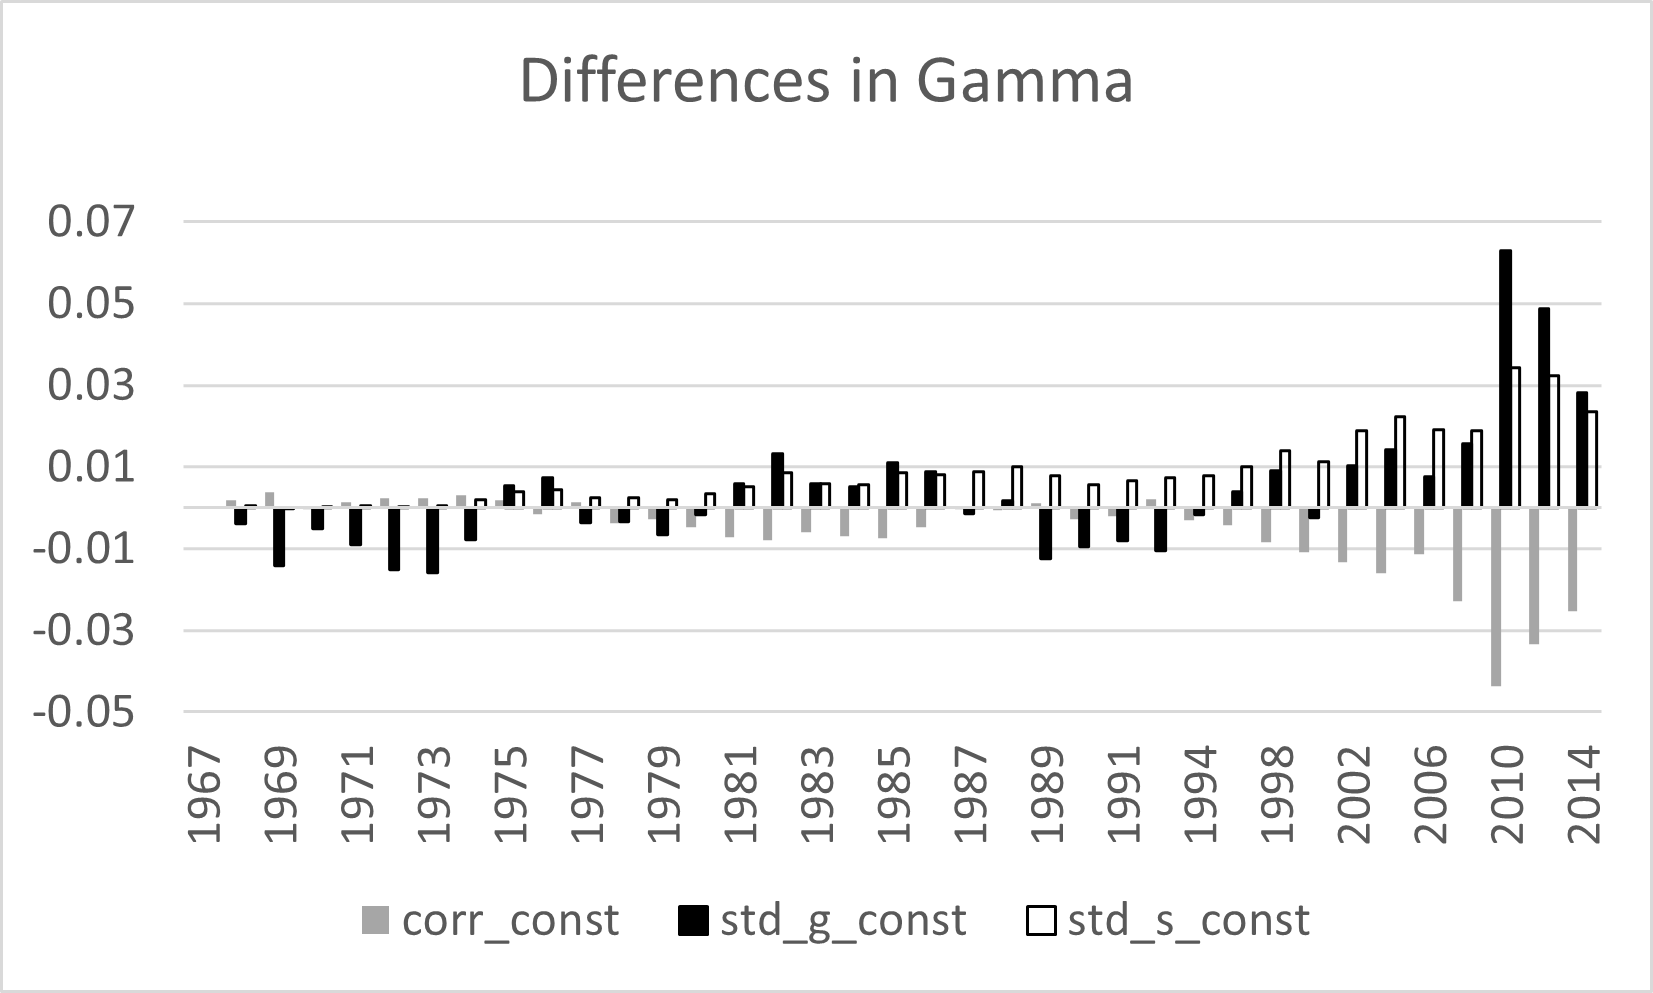
\includegraphics[width=0.48\textwidth]{Figures/Gamma_differences.png}}
  \caption*{}
\end{figure}

\begin{itemize}
    \item Keeping the correlation constant to 1967 level would harm aggregate growth. Correlation has been decreasing in absolute value over time, so by keeping it constant we are imposing high income people to grow less (we have a flatter version of Figure 5). Since high income workers drive aggregate growth, we are reducing aggregate growth by slowing them down.
    \item Keeping the standard deviation of $g$ constant to 1967 levels would generate a higher aggregate growth.
    Volatility has increased over time, so keeping it constant to the 1967 level we are reducing the chances of high growth rates of individual income. 
    \item Keeping the standard deviation of $s$ constant to 1967 levels would generate a higher aggregate growth (confirming the Development Economics literature predictions on income inequality worsening aggregate growth).
\end{itemize}

To understand what keeping the correlation constant to its 1967 level, the following figures show the relation between $s_i$ and $g_i$ in 1967 and 2014 (similar to Figure 5 in the paper). The curve ``2014\_corr1967'' is found using a simple optimization algorithm. The values of $s_i$ and $g_i$ are chosen so that $\sigma(s)$, $\sigma(g)$ and $\mathbb{E}(g)$ are equal to the 2014 levels, while the $corr(s,g)$ has the value of the 1967 curve.
\begin{figure}[H]
  \centering
  \subfloat[Extremes constant]{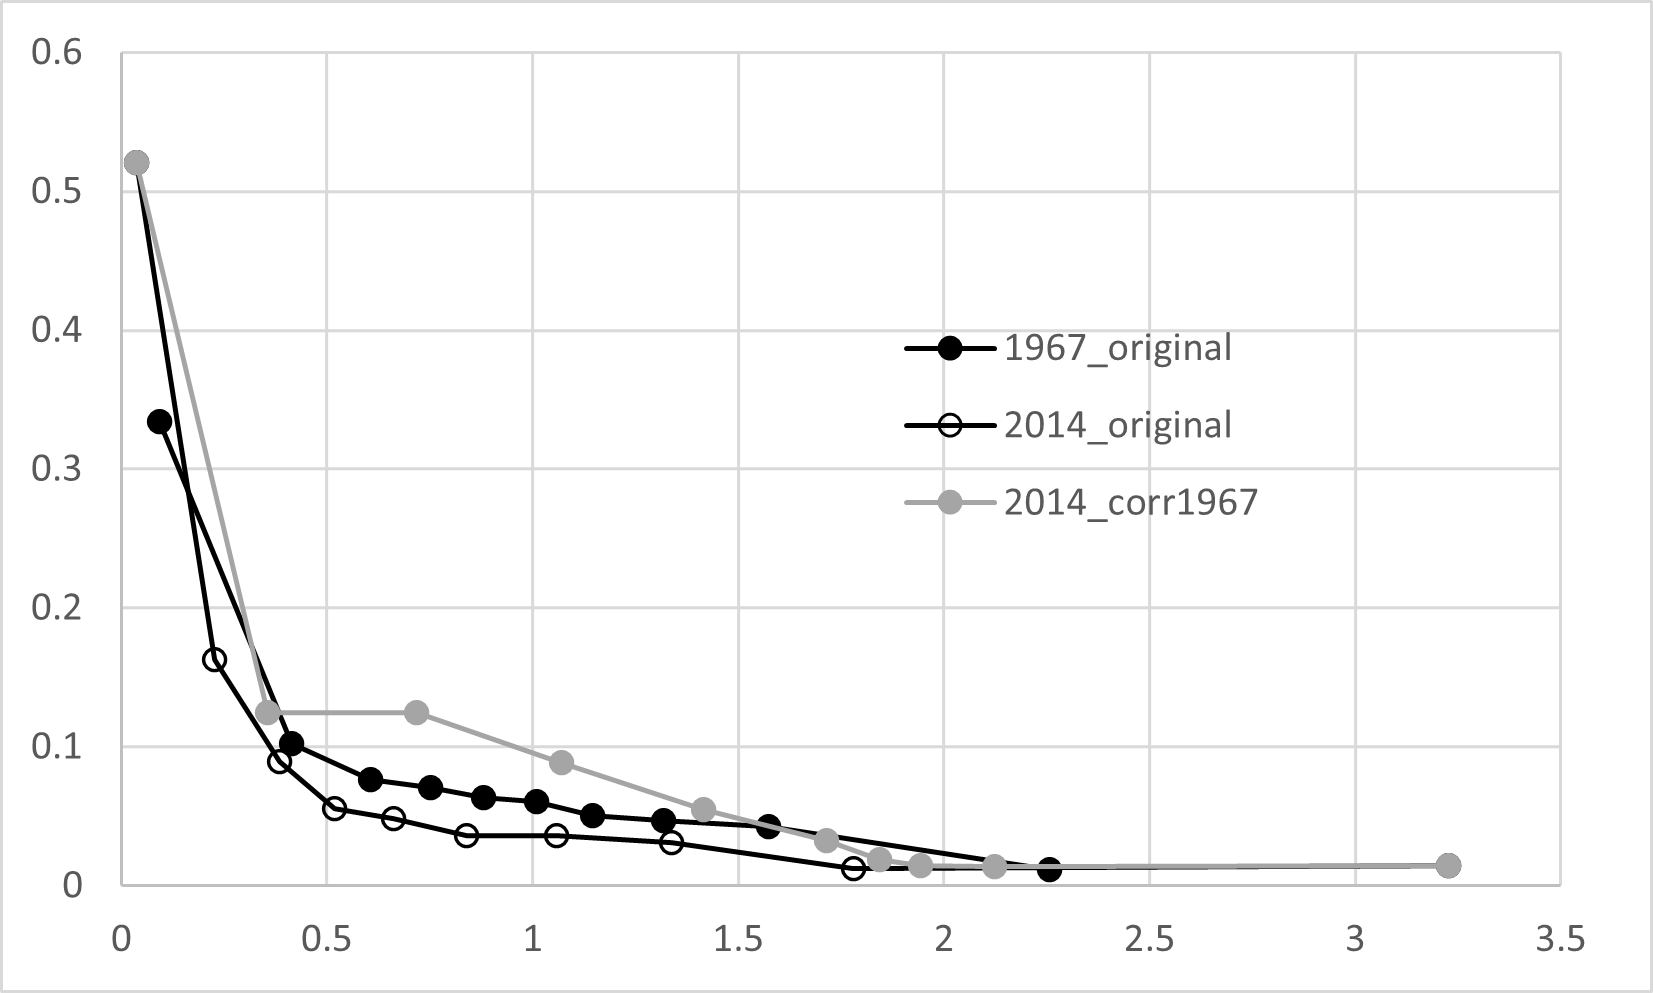
\includegraphics[width=0.7\textwidth]{Figures/Fig5_corr_2014.png}}
  \vfill
  \subfloat[$E(s)=1$, $g_i\geq0$]{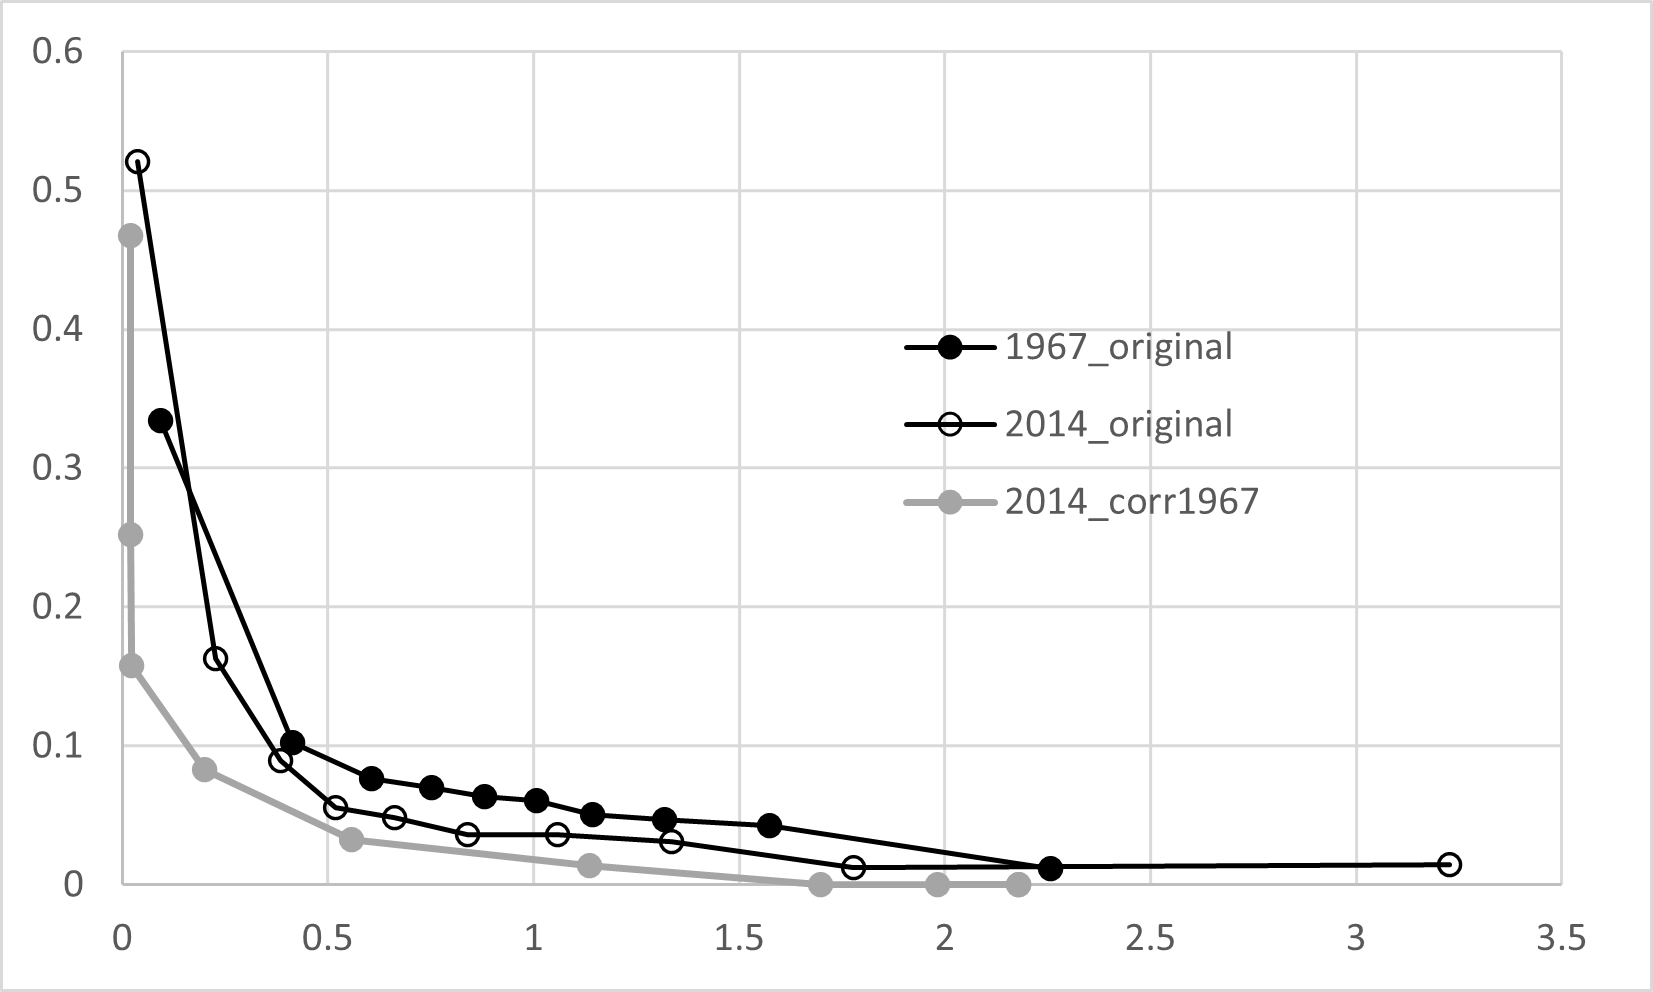
\includegraphics[width=0.7\textwidth]{Figures/Fig5_corr_2014_Es1.png}}
  \caption*{}
  \vfill
  \subfloat[$E(s)=1$]{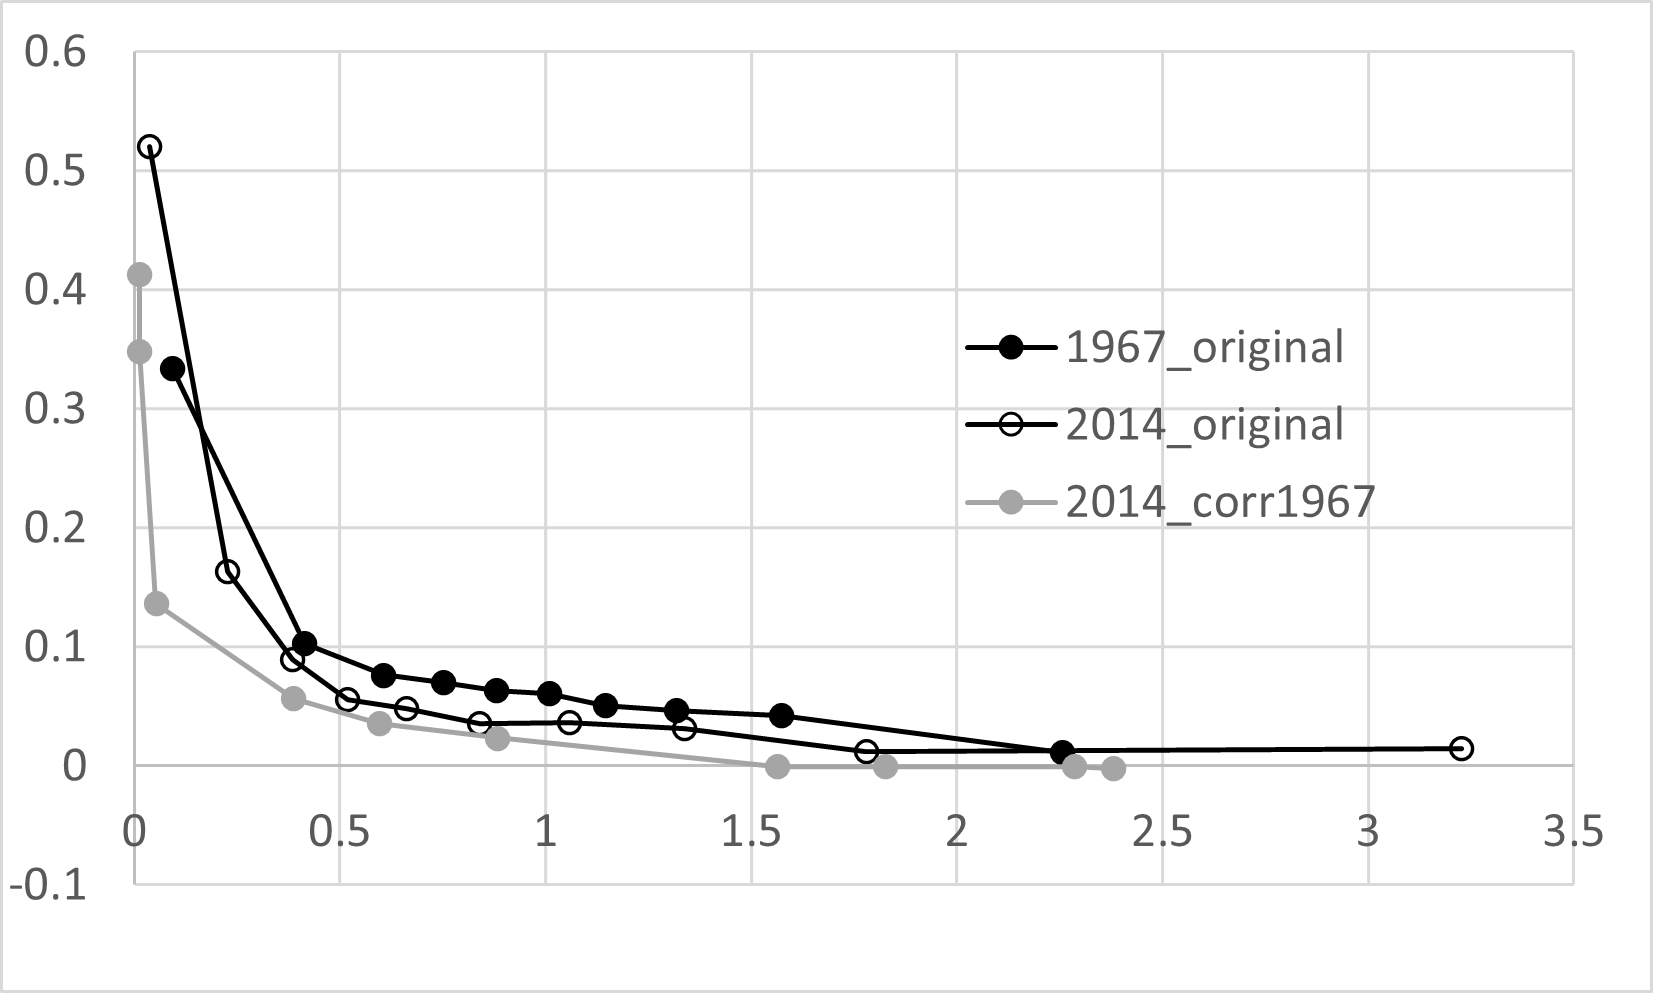
\includegraphics[width=0.7\textwidth]{Figures/Fig5_corr_2014_Es1_V2.png}}
  \caption*{}
\end{figure}



\end{document}
